\chapter{Dislocation-induced surface tractions}
\label{c:tractions}

\Cref{s:numericVsAnalytic} have been adapted from a manuscript prepared for publication. \Cref{s:parallel} outlines the work done in parallelising the analytic traction calculation on GPUs.

\section{Numeric v.s. analytic tractions}\label{s:numericVsAnalytic}

\subsection{Introduction}\label{ss:paperIntro}

In-silico experiments are essential for interpreting experimental data and relating the measured mechanical response to dislocation mechanisms \cite{0965-0393-6-6-007,doi:10.1080/14786430500341250,tarleton2015discrete,YU2018}. Experimentally, we are limited by the electron transparency of the material and our capacity for subjecting samples to representative loads whilst simultaneously keeping dislocations in focus. Modelling, albeit imperfect and idealised, can greatly inform our understanding and provide insight into the dislocation dynamics responsible for our observations.

Simulating micromechanical tests with explicit dislocation interactions necessitates the coupling of discrete dislocation dynamics (DDD) to the finite element method (FEM) \cite{Groh2009}. One of the simples and most popular ways of doing so is the superposition method \cite{superposition_scheme0,superposition_scheme1,superposition_scheme2}. Which works by decomposing the problem into separate DDD and FE problems as illustrated by \cref{f:superposition_scheme}.
\begin{figure}
    \centering
    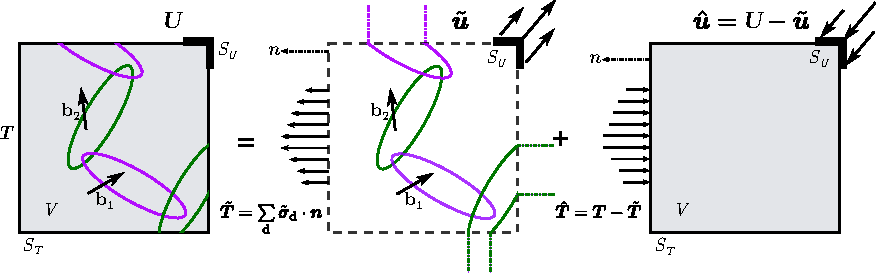
\includegraphics[width=\linewidth]{fem_ddd.pdf}
    \caption[Superposition Model for DDD-FEM coupling.]{The superposition used to couple DDD and FEM. The volume $V$ is bounded by a surface $S = S_{T} \cup S_{U}$ and contains a dislocation ensemble and is subjected to tractions $\vec{T}$ on $S_{T}$ and $\vec{u}$ on $S_{u}$. First, the traction, $\vec{\tilde{T}}$, and displacement, $\vec{\tilde{u}}$, fields due to the dislocations in the infinite domain (DDD) are evaluated on the boundaries $S_{T}$ and $S_{U}$ respectively. Then an elastic boundary value problem can be solved with FEM to calculate the corrective elastic fields required to satisfy the boundary conditions $\vec{\hat{T}} = \vec{T} - \vec{\tilde{T}}$ and $\vec{\hat{u}} = \vec{U} - \vec{\tilde{U}}$.}
    \label{f:superposition_scheme}
\end{figure}

Specifically, a linear-elastic solid $V$ bounded by a surface $S$ is subjected to traction boundary conditions, $\vec{T}$, on $S_{T}$ and displacement boundary conditions, $\vec{U}$, on $S_{U}$. The ($\tilde{~}$) fields are those generated by the dislocations in an infinite solid and in our case are obtained by evaluating analytic solutions in a DDD simulation \cite{a_non-singular_continuum_theory_of_dislocations}. Formally, the dislocation field satisfies,
\begin{align}
     & \left.
    \begin{array}{l}
        \nabla \cdot \tns{\tilde{\sigma}} = \bm{0}                 \\
        \tns{\tilde{\sigma}} = \tns{C} : \tns{\tilde{\varepsilon}} \\
        \tns{\tilde{\varepsilon}} = \frac{1}{2} \left( \nabla \vec{\tilde{u}} + (\nabla \vec{\tilde{u}})^T \right)
    \end{array}
    \right\} \quad \textrm{in V}                                                   \\
    %
     & \tilde{\tns{\sigma}} \cdot \vec{n} = \tilde{\vec{T}} \quad \textrm{on } S_T \\
    %
     & \left.
    \begin{array}{l}
        \vec{\tilde{u}} = U, \quad t>0 \\
        \vec{\tilde{u}} = \bm{0}, \quad t=0
        \label{eq:utildebc}
    \end{array}
    \right\} \quad \textrm{on } S_U \,.
\end{align}
%
As the dislocation fields do not vanish on $S$, the dislocations load the volume by generating tractions, $\tilde{\vec{T}}$, on $S_T$ and displacements, $\vec{\tilde{u}}$, on $S_U$. This additional loading deforms $V$, generating an additional ``image'' stress which the dislocations then feel. Therefore corrective ($\hat{~}$) fields must be superimposed to satisfy the desired boundary conditions. The corrective field which accounts for both the applied and image stress is obtained numerically by solving the elastic boundary value problem,
%
\begin{align}
     & \left.
    \begin{array}{l}
        \nabla \cdot \tns{\hat{\sigma}} = \bm{0}               \\
        \tns{\hat{\sigma}} = \tns{C} : \tns{\hat{\varepsilon}} \\
        \tns{\hat{\varepsilon}} = \frac{1}{2} \left( \nabla \vec{\hat{u}} + (\nabla \vec{\hat{u}})^{T} \right)
    \end{array}\right\} \quad \textrm{in V}                                                  \\
    %
     & \hat{\tns{\sigma}}\cdot\vec{n} = \vec{T} - \tilde{\vec{T}} \quad \textrm{on } S_T \label{eq:thatbc} \\
    %
     & \vec{\hat{u}} = \vec{U} - \vec{\tilde{u}} \quad \textrm{on } S_U \,. \label{eq:uhatbc}
\end{align}
%
Once the solutions to both problems are known, their superposition solves the desired mixed boundary value problem,
%
\begin{align}
     & \left.
    \begin{array}{l}
        \nabla \cdot \tns{\sigma} = \nabla \cdot \left( \tns{\hat{\sigma}} + \tns{\tilde{\sigma}} \right) = \bm{0}                                                              \\
        \tns{\sigma} = \tns{\hat{\sigma}} + \tns{\tilde{\sigma}} = \tns{C} : \left( \tns{\hat{\varepsilon}} + \tns{\tilde{\varepsilon}} \right) = \tns{C} : {\tns{\varepsilon}} \\
        \tns{\varepsilon} = \tns{\hat{\varepsilon}} + \tns{\tilde{\varepsilon}} = \frac{1}{2} \left( \nabla ( \vec{\hat{u}} + \vec{\tilde{u}} ) + \left[ \nabla ( \vec{\hat{u}} + \vec{\tilde{u}} ) \right]^T \right) = \frac{1}{2} \left( \nabla \vec{u} + ( \nabla \vec{u} )^{T} \right)
    \end{array}
    \right\}\quad \textrm{in V}                                    \\
    %
     & \tns{\sigma} \cdot \vec{n} = \vec{T} \quad \textrm{on } S_T \\
    %
     & \left.
    \begin{array}{l}
        \vec{u} = \vec{U}, \quad t>0 \\
        \vec{u} = \bm{0}, \quad t=0
    \end{array}
    \right\} \quad \textrm{on } S_U
    \label{eq:ubc}
\end{align}

For all its simplicity and elegance, the method is not without issue. As the distance between dislocation and surface decreases, $\tns{\tilde{\sigma}}$ diverges \cite{boundary_problems_in_dd}. This can be partially solved by using a non-singular formulation for $\tns{\tilde{\sigma}}$, such as that proposed by \citet{a_non-singular_continuum_theory_of_dislocations}. Regardless, the steep gradients in the dislocation field are difficult to accurately capture as the dislocation approaches $S$. Another problem with this method is the large computational cost when simulating a heterogeneous solid, as this requires calculating polarisation stresses due to the difference in the elastic constants between phases \cite{superposition_scheme0,boundary_problems_in_dd,ddd_precipitate}.

A modified superposition scheme \cite{ODay2004} can overcome this by dividing the problem into separate DDD-FEM problems coupled through a elastic FE problem. This requires accurate evaluation of $\vec{\tilde{T}}$ on the domain boundaries---which can only be captured with a fine FE mesh---increasing the computational cost. Therefore, simulating polycrystalline or composite materials using superposition necesitates methods to accurately evaluate both $\vec{\tilde{u}}$ and $\vec{\tilde{T}}$. The displacements can be evaluated analytically as shown by \cite{bromage2018calculating} and this paper investigates the evaluation of the dislocation tractions analytically.

As previously mentioned, the relative simplicity of the superposition method has made it a popular choice for coupling DDD and FEM as all it needs is the evaluation of FE nodal forces and displacements on the boundary. Furthermore, the analytic expression for the stress field produced by a finite, straight dislocation line segment has allowed \citet{analytic_tractions} to use the non-singular formulation \cite{a_non-singular_continuum_theory_of_dislocations} to obtain closed-form solutions for the tractions generated by the segment on the surface of a finite element.

\subsection{Theory}\label{ss:paperTheory}

The force exerted by a dislocation ensemble on a node, $a$, belonging to element, $e$, is given by,
%
\begin{align}
    \vec{F}_{a} = \int_{S_{e}} \left[\tns{\tilde{\sigma}}(\vec{x}) \cdot \vec{n}\right] N_{a}(\vec{x})\; \mathrm{d}S_{e}\,.
    \label{eq:ddd_fem_force}
\end{align}
%
Where $\mathrm{d}S_{e}$ is the surface of element $e$ with surface area $S_{e}$, and $N_{a}$ is the finite element shape function for node $a$. The solutions are for linear rectangular surface elements and as such the shape functions are,
\begin{align}
    \label{eq:shape_function}
    N_{1} & = \dfrac{1}{4}(1-s_1)(1-s_2)             \\
    N_{2} & = \dfrac{1}{4}(1+s_1)(1-s_2)\nonumber    \\
    N_{3} & = \dfrac{1}{4}(1+s_1)(1+s_2)\nonumber    \\
    N_{4} & = \dfrac{1}{4}(1-s_1)(1+s_2)\nonumber\,.
\end{align}
Where $s_1$ and $s_2$ are the orthogonal coordinates local to the element.

Gauss quadrature is usually used to numerically evaluate the surface integral in \cref{eq:ddd_fem_force}. In 1D this is,
%
\begin{align}
    \label{eq:gauss_leg}
    \int\limits_{-1}^{1} f(s)\;\mathrm{d}s \approx \sum\limits_{i=1}^{n} w_{i} f(s_{i}) \quad \textrm{where}\quad
    %
    w_{i} = \dfrac{2}{\left(1-s_{i}^{2}\right) \left[P_{n}^{'}\left(s_{i}\right)\right]^{2}}\,,
\end{align}
%
is the weighting of the Gauss point, $s_{i}$, which is the $i\textsuperscript{th}$ root of the $n\textsuperscript{th}$ normalised Legendre polynomial, $P_{n}(1) = 1$. $P_{n}^{'}$ is the first order derivative of $P_{n}$. This method is very accurate for functions that can be accurately approximated by polynomials. In fact, for a polynomial of degree $n$, one needs $n-1$ points to obtain an exact numerical solution. However, this quadrature is well-known for being unsuitable for integrating functions with poles or near-poles \cite{gauss_leg, gauss_leg_sing}.

We avoid the strict pole in $\tns{\tilde{\sigma}}$ by using the non-singular formulation described in \cite{a_non-singular_continuum_theory_of_dislocations}, where the true singularity is avoided by adding a small cut-off radius to account for the dislocation core. However, if an integration point falls close to, or within the dislocation core, Gauss quadrature can still produce large errors.

For rectangular surface elements, we must transform from the parent element in $(s_1,\,s_2)$ in \cref{eq:gauss_leg} to the real element coordinate system $(x\,,y\,,z)$. Evaluating \cref{eq:ddd_fem_force} in the parent element and mapping to the real element gives the force on node $a$,
\begin{align}
    \label{eq:gauss_leg_ddd_fem_force}
    \vec{F}_{a} \approx \sum\limits_{i=1}^{Q} w_{i} \sum\limits_{j=1}^{Q} w_{j} [\tns{\tilde{\sigma}}(r_{i}, s_{j})\cdot \vec{n}] N_{a}(r_{i}, s_{j}) \det(\mtx{J})\,.
\end{align}
Where the sum is over the $Q$ quadrature points and $J_{ij} = dx_{i}/ds_{j}$, is the element Jacobian defining the transformation from $(s_1,\,s_2) \mapsto (x,\,y)$. Since the real element is rectangular with surface area $S_e$, then $\det(\mtx{J}) = S_e/4$. \Cref{f:2d_gaussian_quad} contains examples of how the Gauss points are distributed on the surface.
\begin{figure}
    \centering
    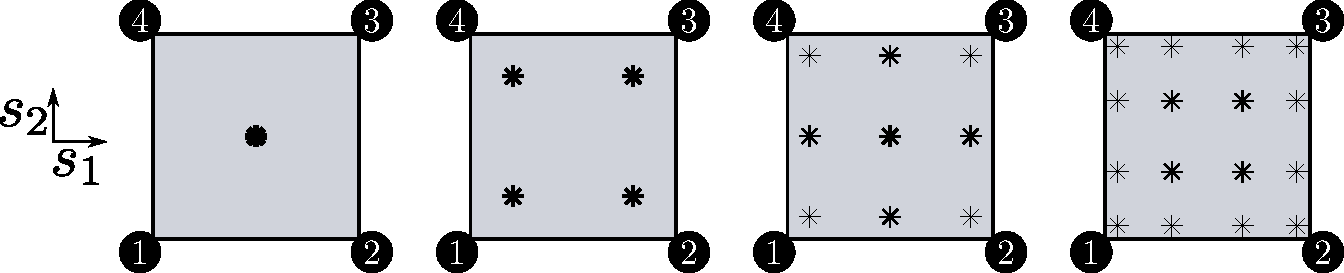
\includegraphics[width=\linewidth]{2d_gaussian_quad.pdf}
    \caption[2D Gauss-Legendre quadrature on quadrangles.]{Examples of 2D Gauss-Legendre quadrature of the parent element with $Q = 1,\, 2,\, 3,\, 4$. The point size represents the weight $w$ of the integration point. The parent elements are centred at the origin and $s_1,\, s_2 \in [-1,\,1]$. We use an anticlockwise node numbering scheme.}
    \label{f:2d_gaussian_quad}
\end{figure}

\begin{figure}
    \centering
    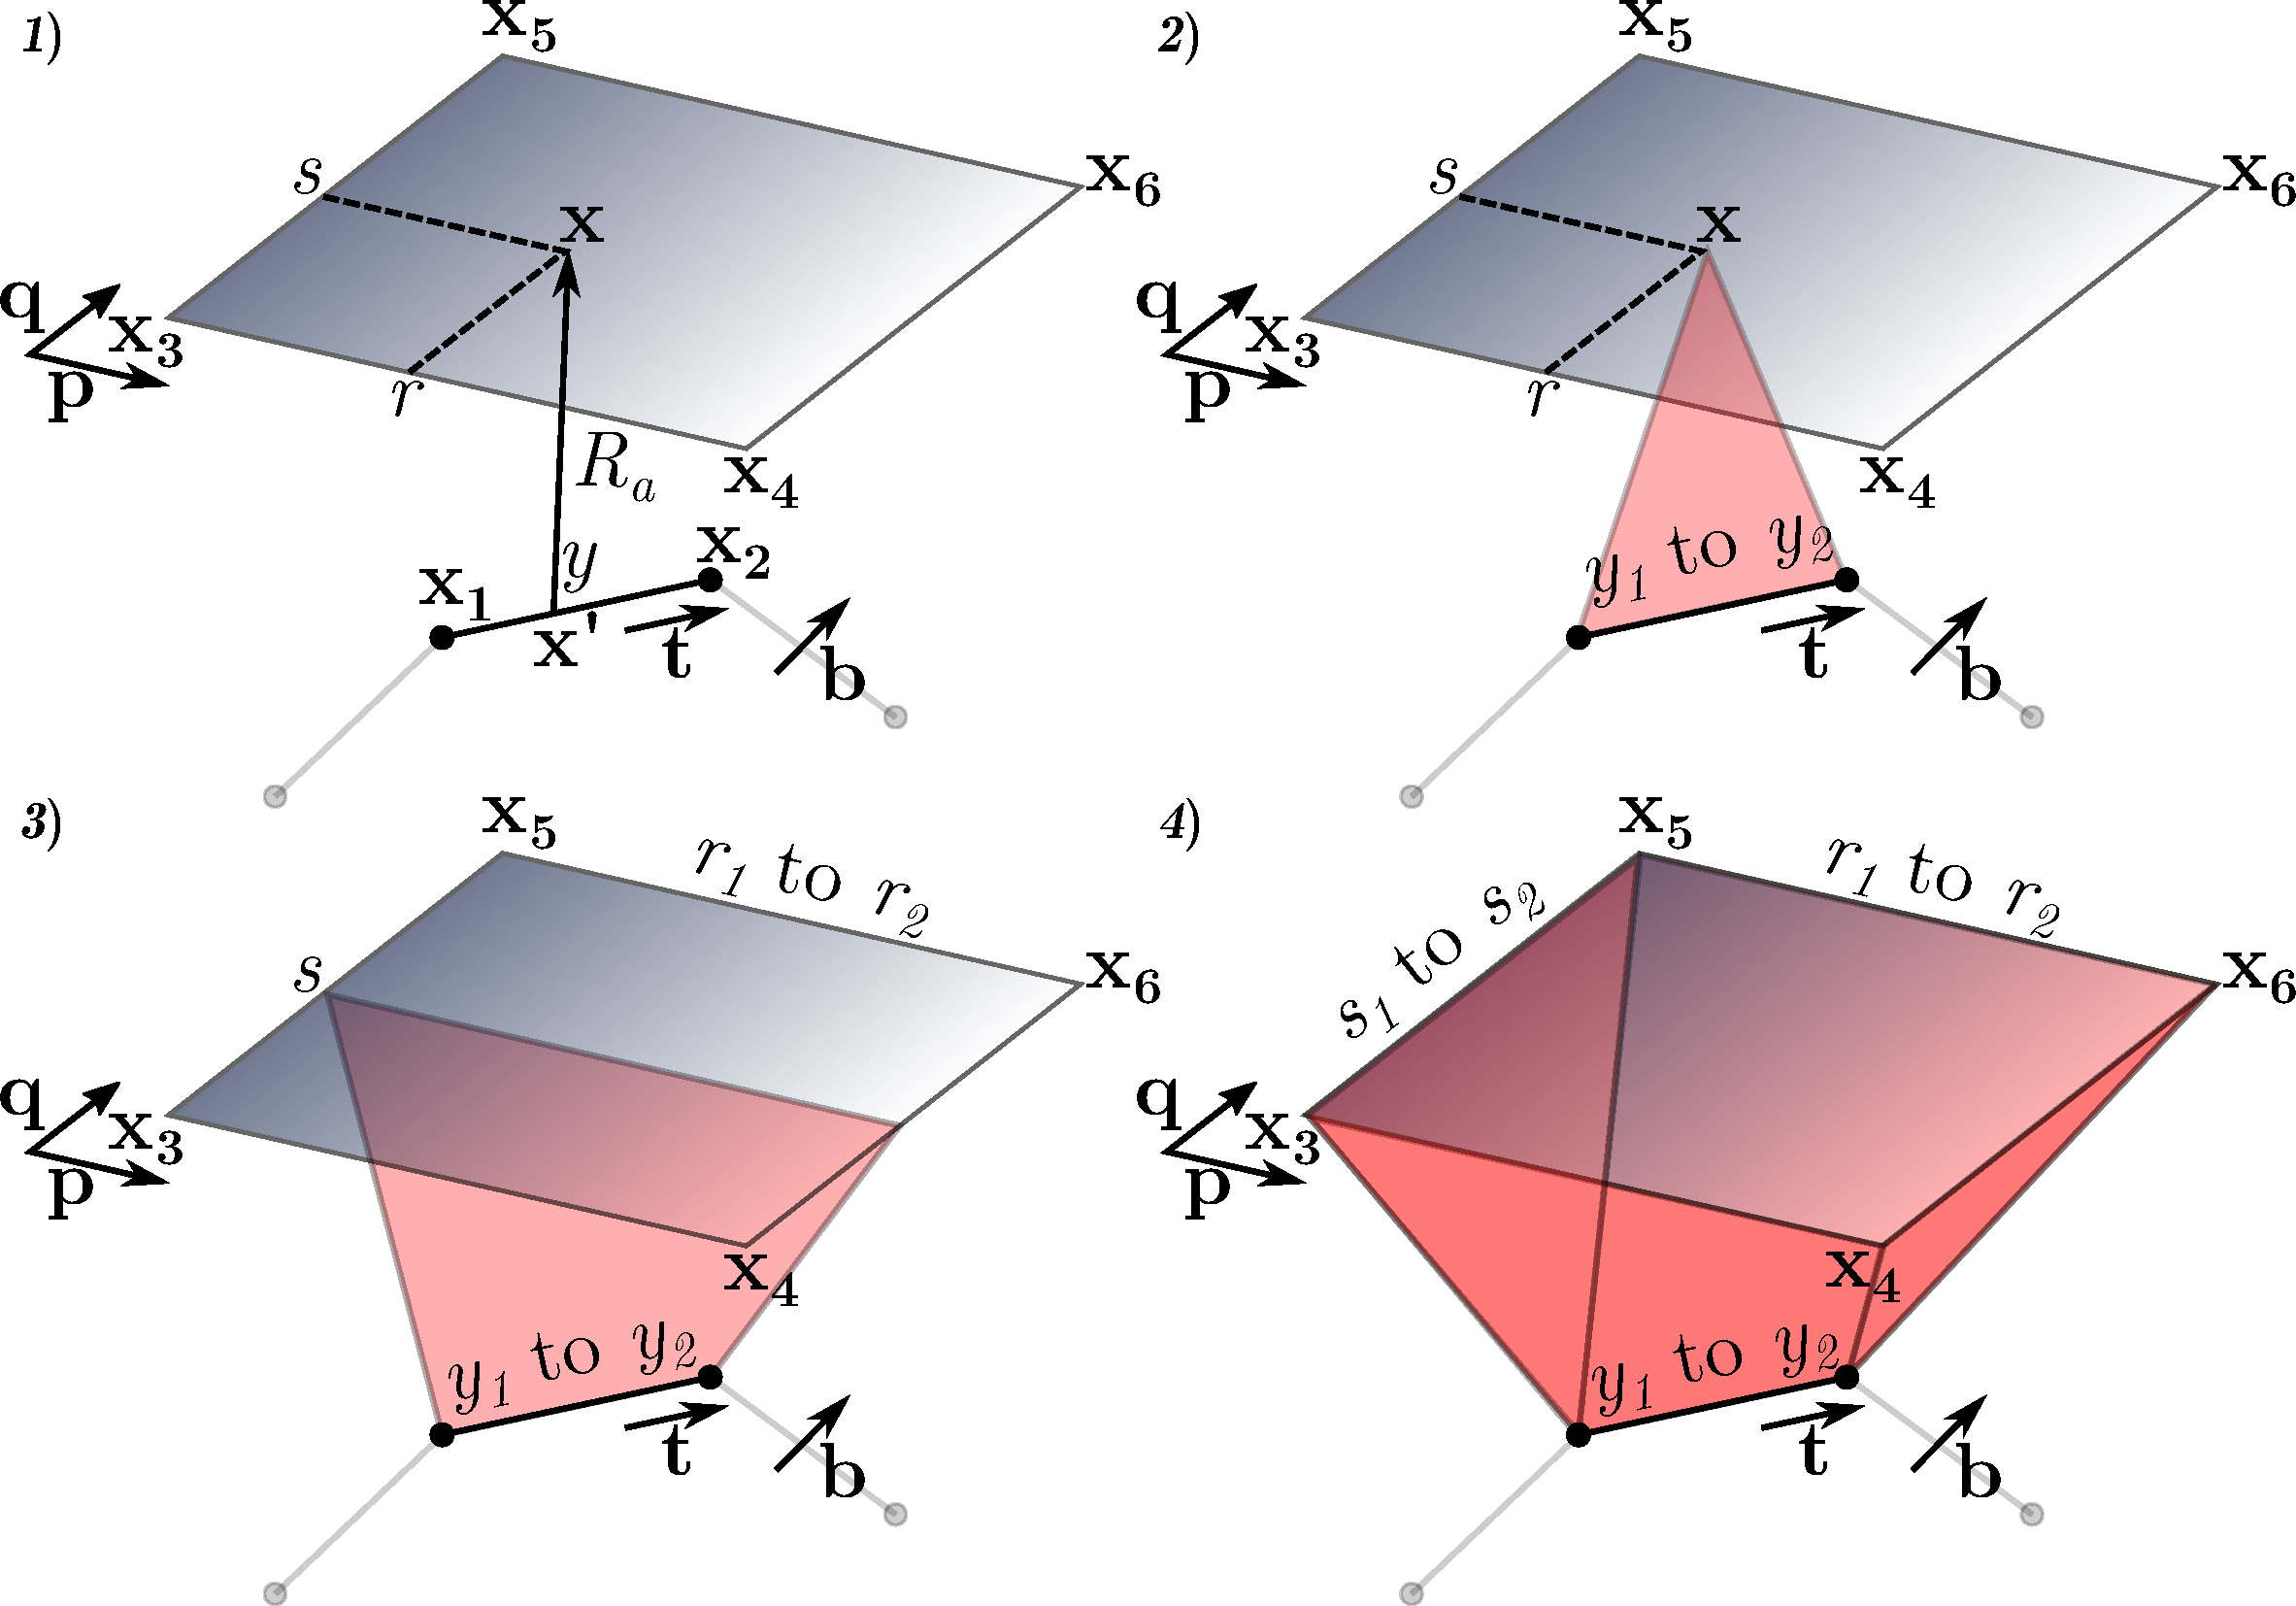
\includegraphics[width=0.8\linewidth]{force_calc_linear_rectangle.pdf}
    \caption[Analytic tractions on linear rectangular surface elements.]{Diagram of the parametric line integrals solved by \citet{analytic_tractions} to find the forces on linear rectangular surface elements.}
    \label{f:force_lin_rect}
\end{figure}
Explicitly, \cref{eq:ddd_fem_force} is actually a triple vector integral as shown in \cref{f:force_lin_rect}. This is because given the isotropic Burgers vector distribution proposed in \cite{a_non-singular_continuum_theory_of_dislocations}, the dyadic form of the stress tensor produced by a straight, finite dislocation segment bounded by nodes at $\mathbf{x_1}$ and $\mathbf{x_2}$ \cite{analytic_tractions} is,
\begin{align}
    \label{eq:stress}
    \tns{\tilde{\sigma}}(\vec{x}) = &
    - \dfrac{\mu}{8\pi} \int\limits_{\mathbf{x_1}}^{\mathbf{x_2}} \left( \dfrac{2}{R_{a}^{3}} + \dfrac{3a^2}{R_{a}^{5}} \right) \left[ \left(\vec{R} \times \vec{b}\right) \otimes \mathrm{d}\vec{x'} + \mathrm{d}\vec{x'} \otimes \left(\vec{R} \times \vec{b}\right) \right]          \\
    %
                                    & + \dfrac{\mu}{4\pi(1-\nu)} \int\limits_{\mathbf{x_1}}^{\mathbf{x_2}} \left( \dfrac{1}{R_{a}^{3}} + \dfrac{3a^2}{R_{a}^{5}} \right) \left[ \left(\vec{R} \times \vec{b}\right) \cdot \mathrm{d}\vec{x'} \right]\vec{I_2}\nonumber                  \\
    %
                                    & -\dfrac{\mu}{4\pi(1-\nu)} \int\limits_{\mathbf{x_1}}^{\mathbf{x_2}}  \dfrac{1}{R_{a}^{3}} \left[ \left(\vec{b} \times \mathrm{d}\vec{x'}\right) \otimes \vec{R} + \vec{R} \otimes \left(\vec{b} \times \mathrm{d}\vec{x'}\right) \right]\nonumber \\
    %
                                    & + \dfrac{\mu}{4\pi(1-\nu)} \int\limits_{\mathbf{x_1}}^{\mathbf{x_2}} \dfrac{3}{R_{a}^{5}} \left[ \left(\vec{R} \times \vec{b}\right) \cdot \mathrm{d}\vec{x'} \right]\vec{R}\otimes\vec{R}\nonumber,
\end{align}
where,
\begin{align}
    \vec{R}            & = \vec{x} - \vec{x'} = y \vec{l} + r \vec{p} + s \vec{q} \\
    %
    R_a                & = \sqrt{\vec{R} \cdot \vec{R} + a^2}                     \\
    %
    \mathrm{d}\vec{x'} & = -\mathrm{d} y \vec{l}\,.
\end{align}
The vectors $\vec{p}$ and $\vec{q}$ are aligned with the edges of the rectangular finite element, $\vec{n} = \vec{p} \times \vec{q}$ is the element surface normal (pointing away from the dislocation), and $\vec{l}$ is parallel to the dislocation line segment as shown in \cref{f:force_lin_rect}. Then (provided $\vec{l}$ is not parallel to $\vec{p}$ or $\vec{q}$) $\vec{R}$ can be expressed in terms of $(\vec{l},~\vec{p},~\vec{q})$ with coefficients,
\begin{align}
    y = \dfrac{\vec{R}\cdot \vec{n}}{\vec{l}\cdot \vec{n}} \label{eq:problem},\quad
    %
    r = \dfrac{\vec{R}\cdot (\vec{q} \times \vec{l})}{\vec{p}\cdot (\vec{q} \times \vec{l})}, \quad
    %
    s = \dfrac{\vec{R}\cdot (\vec{p} \times \vec{l})}{\vec{q}\cdot (\vec{p} \times \vec{l})}\,.
\end{align}

Substituting \cref{eq:stress} and \cref{eq:shape_function} into \cref{eq:ddd_fem_force} yields four long and messy equations (one for each FE node) that were elegantly solved by \citet{analytic_tractions} by utilising the fact that the triple integrals all had the form,
\begin{align}
    H_{ijkl}        & = \int\limits_{r_{1}}^{r_{2}}\int\limits_{s_{1}}^{s_{2}}\int\limits_{y_{1}}^{y_{2}} \dfrac{r^i s^j y^k}{R_{a}^{m}}\label{eq:triple_int} \\
    \textrm{when }m & = 5 \textrm{ then } i,\, j \in [0,\,3],~k \in [0,\,2]\nonumber                                                                          \\
    \textrm{when }m & = 3 \textrm{ then } i,\, j \in [0,\,2],~k \in [0,\,1]\nonumber                                                                          \\
    \textrm{when }m & = 1 \textrm{ then } i = j = k = 0\,.
\end{align}
Using partial differentiation and integration by parts, they found a series of recurrence relations that lead to double and single integrals of similar form to \cref{eq:triple_int}. All of which are used to construct a full, exact solution. The recurrence relations stop working when $i = j = k = 0 \textrm{ and } m = 1,\, 3$. At which point, direct integration of the remaining single and double integrals (the last triple integrals all cancel out in the global calculation) yields six seed functions that are used as the starting point for the recurrence relations. Three of them are logarithms and three either arctangents or---if a discriminant is negative---hyperbolic arctangents. The details of the procedure can be found in \cite{analytic_tractions}.

Although exact, the use of arctangents, hyperbolic arctangents and logarithmic functions, compounded by the large number of recurrence relations is prime territory for error propagation and numerical problems (see \cref{ss:paperMethod}). The problem is particularly egregious when using general purpose compilers instead of high-performance or scientific computing compilers where mathematical functions are implemented more precisely. Such issues must be taken into account when using analytic tractions, which can be done by using numerical tolerances as described in \cref{ss:paperMethod}.

In simulations, tractions are manifested as image stresses calculated by the FE solver at FE nodes. In order to validate and compare the practical differences between analytic and numeric methods, we compare the resulting image stresses from both methods to the analytic expressions for infinite dislocations in inhomogenous media for edge dislocations \cite{head1953edge}, as well as those for screw dislocations \cite[p.~59,~64]{hirth1983theory}. We keep the same nomenclature and coordinate system as both infinite-domain solutions. Where the traction surface is the line $x=0$, the dislocation line direction is the positive $z$-direction (pointing out of the page), the dislocation coordinates are represented by $(a,~c)$, and points in the $xy$-plane described by their $(x,\,y)$ coordinates.

The original paper by \citet{head1953edge} has a few typos that have been replicated in other sources. We therefore include the complete and correct expressions in \cref{eq:imageStressAnalyticEdge1,eq:imageStressAnalyticEdge2,eq:imageStressAnalyticScrew}. \citet{head1953edge} gives two basic cases. \Cref{eq:imageStressAnalyticEdge1} corresponds to the case where $\vec{b}$ is perpendicular to the surface and positive $b$ means it points in the positive $x$-direction,
\begin{subequations}\label{eq:imageStressAnalyticEdge1}
    \begin{align}
        \sigma_{xx} = D (y - c) & \left\{-\dfrac{3 (x - a)^2 + (y - c)^2}{[(x - a)^2 + (y - c)^2]^2} + \dfrac{3 (x + a)^2 + (y - c)^2}{[(x + a)^2 + (y - c)^2]^2}\right.                                             \\\nonumber
                                & \left. + 4 a x \dfrac{3 (x + a)^2 - (y - c)^2}{[(x + a)^2 + (y - c)^2]^3}\right\}\,,                                                                                               \\
        \sigma_{yy} = D (y - c) & \left\{\dfrac{(x - a)^2 - (y - c)^2}{[(x - a)^2 + (y - c)^2]^2} - \dfrac{(x + a)^2 - (y - c)^2}{[(x + a)^2 + (y - c)^2]^2}                                                 \right. \\\nonumber
                                & \left. + 4 a (2 a - x) \dfrac{(x + a)^2 + (3 x + 2 a) (y - c)^2}{[(x + a)^2 + (y - c)^2]^3}\right\}\,,                                                                             \\
        \sigma_{xy} = D         & \left\{(x - a) \dfrac{(x - a)^2 - (y - c)^2}{[(x - a)^2 + (y - c)^2]^2} - (x + a) \dfrac{(x + a)^2 - (y - c)^2}{[(x + a)^2 + (y - c)^2]^2}\right.                                  \\\nonumber
                                & \left. + 2 a \dfrac{6 x (x + a) (y - c)^2 - (x - a) (x + a)^3 - (y - c)^4}{[(x + a)^2 + (y - c)^2]^3}\right\}\,.
    \end{align}
\end{subequations}
\Cref{eq:imageStressAnalyticEdge2} corresponds to the case where the $\vec{b}$ lies parallel to the surface and positive $b$ means it points in the positive $y$-direction,
\begin{subequations}\label{eq:imageStressAnalyticEdge2}
    \begin{align}
        \sigma_{xx} = D         & \left\{ (x - a) \dfrac{(x - a)^2 - (y - c)^2}{[(x - a)^2 + (y - c)^2]^2} -(x + a) \dfrac{(x + a)^2 - (y - c)^2}{[(x + a)^2 + (y - c)^2]^2} \right.     \\\nonumber
                                & \left. + 2 a \dfrac{(3 x + a) (x + a)^3 - 6 x (x + a) (y - c)^2 - (y - c)^4}{[(x + a)^2 + (y - c)^2]^3}\right\}\,,                                     \\
        \sigma_{yy} = D         & \left\{ (x - a) \dfrac{(x - a)^2 + 3 (y - c)^2}{[(x - a)^2 + (y - c)^2]^2} - (x + a) \dfrac{(x + a)^2 + 3 (y - c)^2}{[(x + a)^2 + (y - c)^2]^2}\right. \\\nonumber
                                & \left. - 2 a \dfrac{(x - a) (x + a)^3 - 6 x (x + a) (y - c)^2 + (y - c)^4}{[(x + a)^2 + (y - c)^2]^3}\right\}\,,                                       \\
        \sigma_{xy} = D (y - c) & \left\{\dfrac{(x - a)^2 - (y - c)^2}{[(x - a)^2 + (y - c)^2]^2} - \dfrac{(x + a)^2 - (y - c)^2}{[(x + a)^2 + (y - c)^2]^2} \right.                     \\\nonumber
                                & \left. + 4 a x \dfrac{3 (x + a)^2 - (y - c)^2}{[(x + a)^2 + (y - c)^2]^3}\right\}\,.
    \end{align}
\end{subequations}
\Cref{eq:imageStressAnalyticScrew} corresponds to screw dislocations, which are markedly simpler as only the shear components are non-zero. Here $\vec{b} = \vec{l}$ so positive $b$ means it points in the positive $z$-direction,
\begin{subequations}\label{eq:imageStressAnalyticScrew}
    \begin{align}
        \sigma_{xz} & = -D \left(\dfrac{y - c}{(x - a)^2 + (y - c)^2} - \dfrac{y - c}{(x + a)^2 + (y - c)^2}\right)   \\
        \sigma_{yz} & = D \left(\dfrac{x - a}{(x - a)^2 + (y - c)^2} - \dfrac{x + a}{(x + a)^2 + (y - c)^2}\right)\,.
    \end{align}
\end{subequations}
In every case, the constant $D$ is defined by \cref{eq:Dconstant},
\begin{align}\label{eq:Dconstant}
    D = \dfrac{\mu}{2\pi} \cdot \dfrac{1+\nu}{1-\nu^2} \cdot b\,.
\end{align}
Note the first terms of \cref{eq:imageStressAnalyticEdge1,eq:imageStressAnalyticEdge2,eq:imageStressAnalyticScrew} all correspond to the stress field generated by the dislocation itself. The following terms are the corrective terms required to make the boundary conditions on the surface equal to zero. Therefore, we can split these equations and only look at the real or corrective terms independently, which we do in order to only visualise the effect of the different traction calculations. Furthermore, \cref{eq:imageStressAnalyticEdge1,eq:imageStressAnalyticEdge2,eq:imageStressAnalyticScrew} are all singular at the dislocation coordinates. Our simulation code uses the non singular expressions found by \citet{a_non-singular_continuum_theory_of_dislocations}, which smooth out drastic increases in stresses and avoid numerical blow up as we near the dislocation core.

\subsection{Methodology}\label{ss:paperMethod}

Numerical integration of tractions can produces unexpected behaviour such as force hot spots and sign inversions as a dislocation approaches a surface. During a large simulation, these effects are hard to spot. \Cref{f:err_basic_cantilever} has a quick example of the relative errors for an idealised system not disimilar to what can be found with in a simple cantilever bending simulation with a single dislocation loop. As expected, the errors decrease as the mesh gets finer.
\begin{figure}
    \centering
    \subfloat[$60 \times 16$ elements ($x \times y$).]
    {
        { 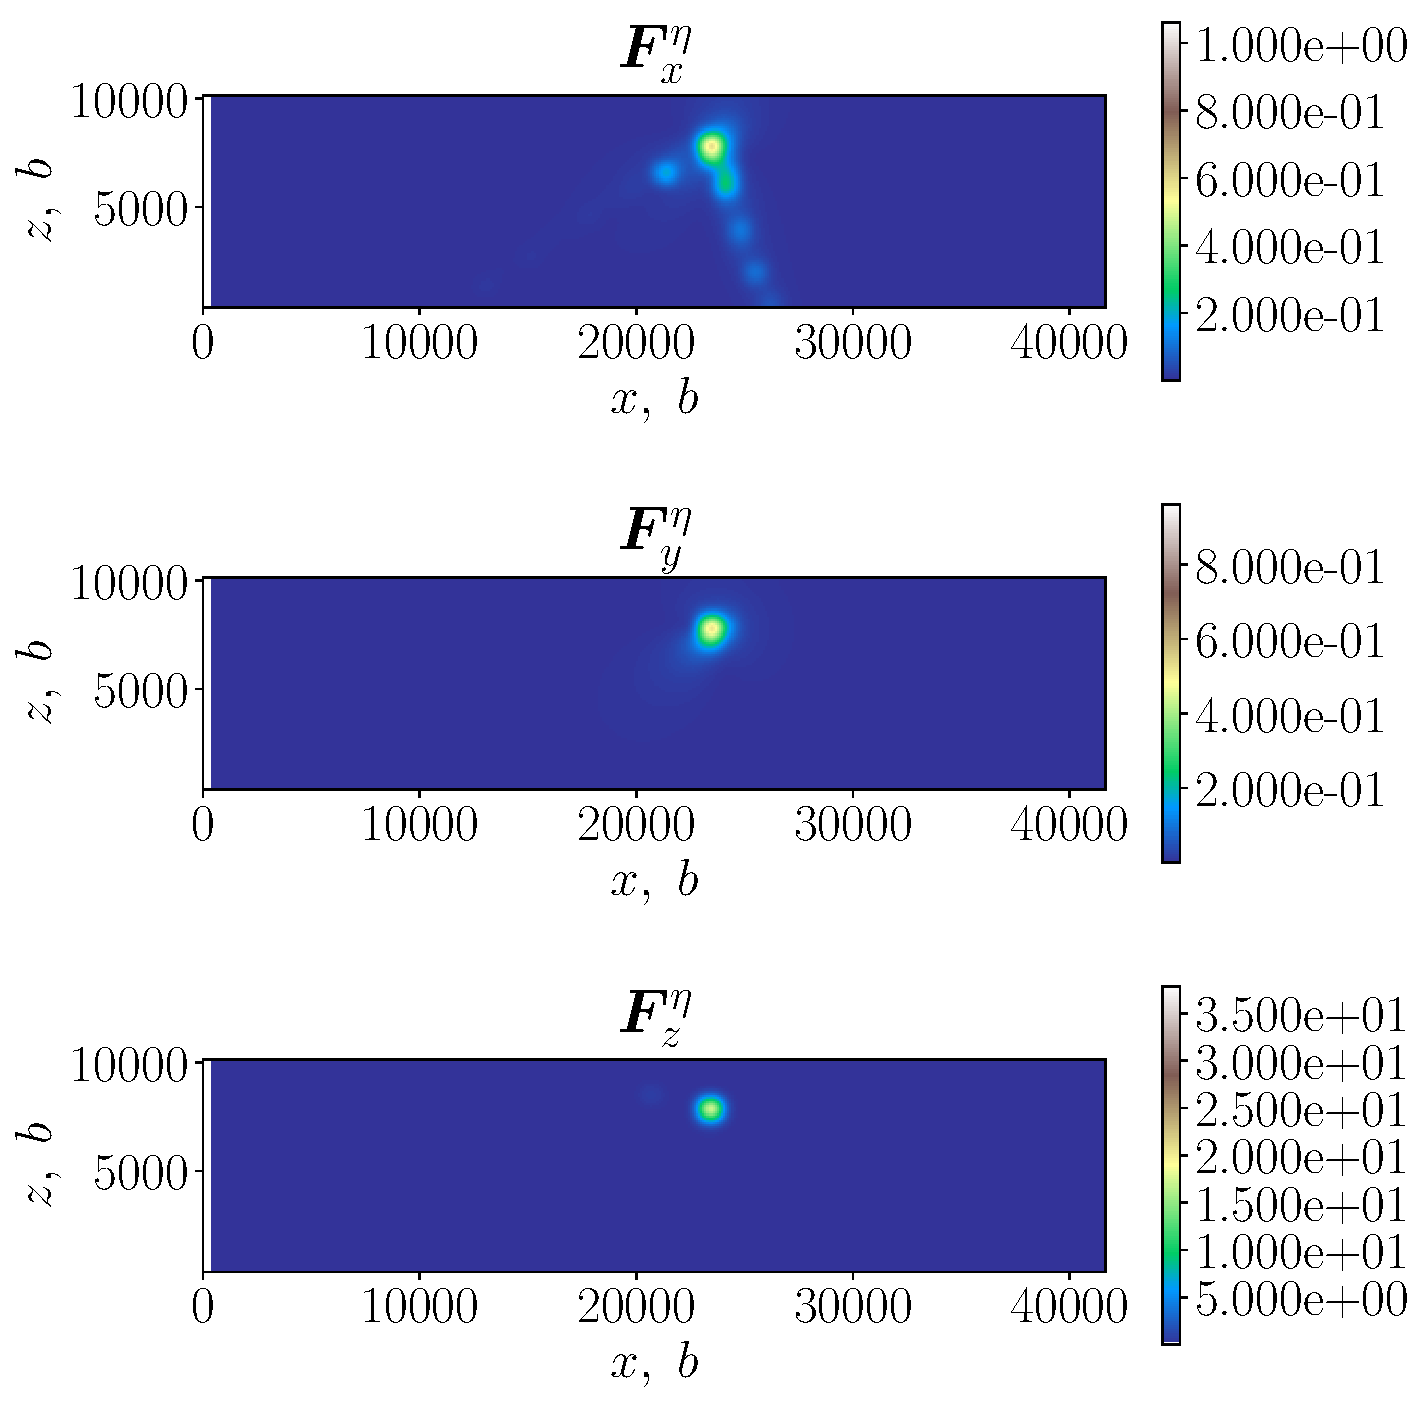
\includegraphics[width=0.45\linewidth]{eta_mx=60_face=1.pdf} }
    }
    ~
    \subfloat[$120 \times 36$ elements ($x \times y$).]
    {
        { 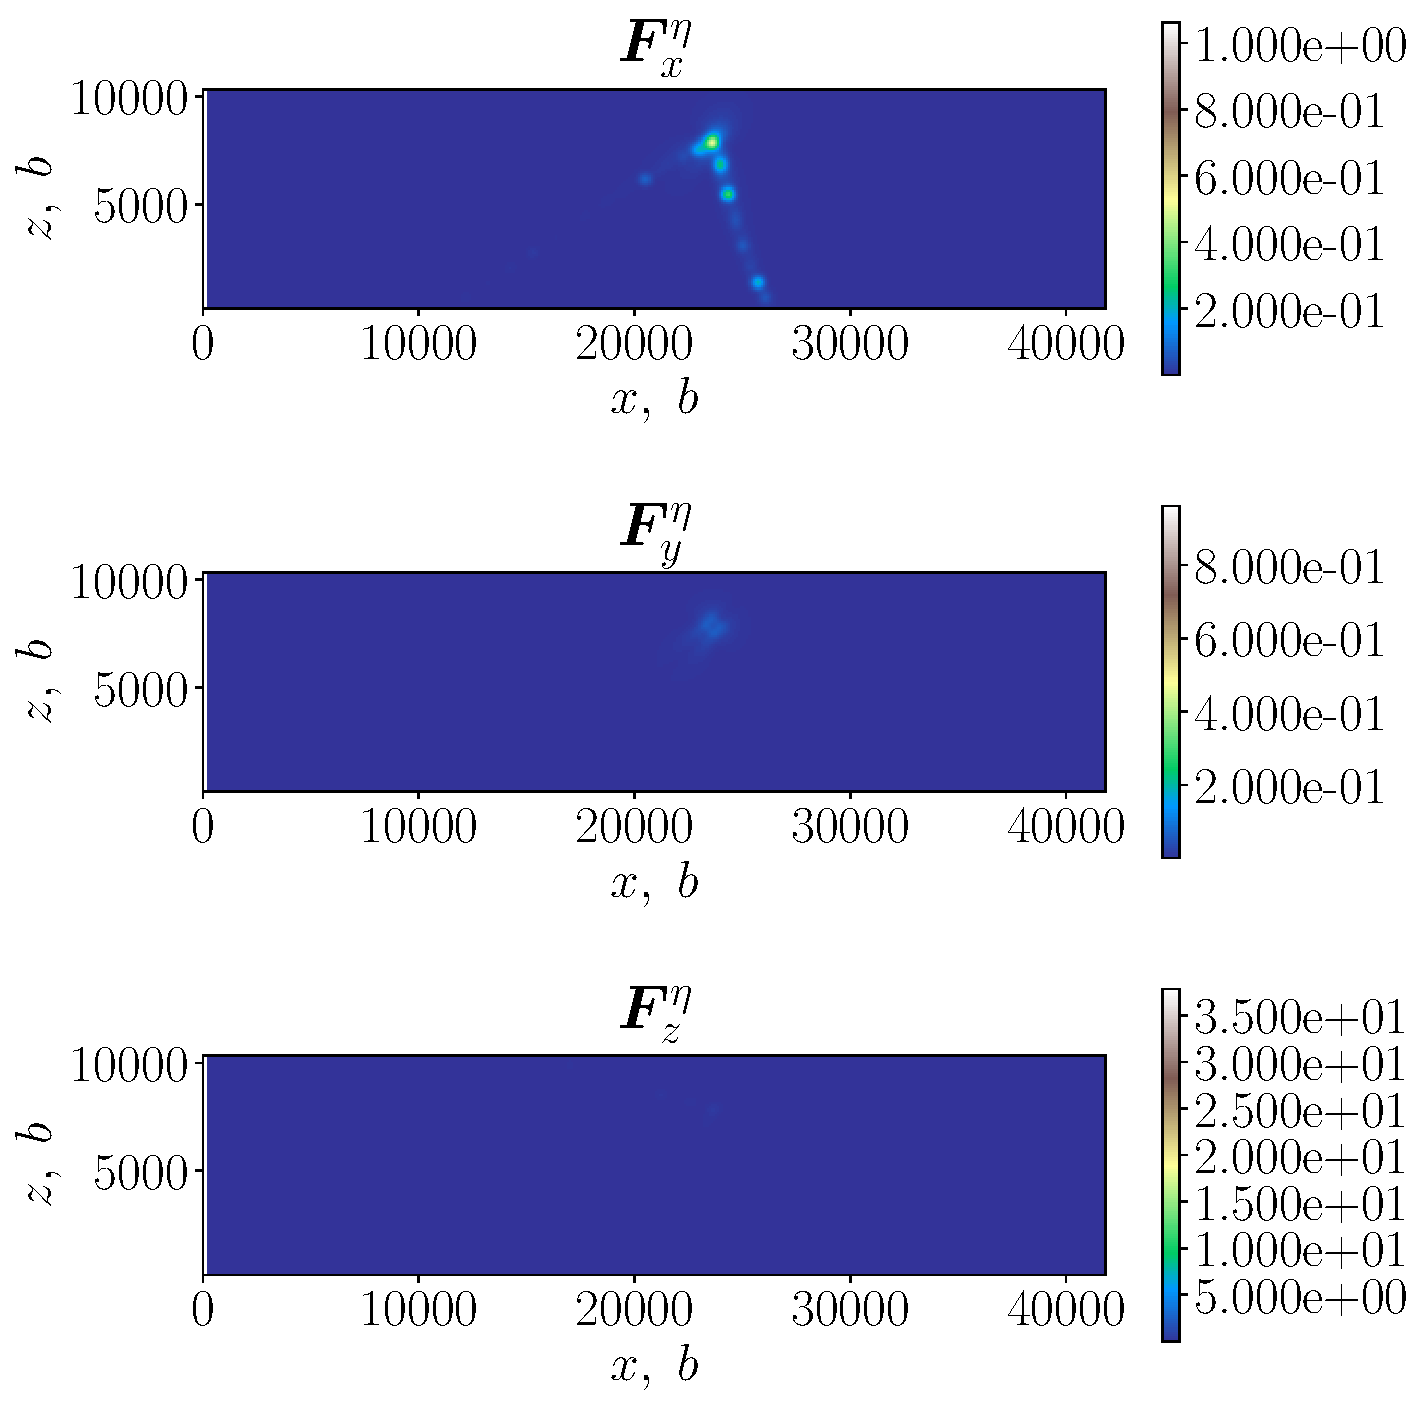
\includegraphics[width=0.45\linewidth]{eta_mx=120_face=1.pdf} }
    }
    \caption[Relative error comparison of analytic v.s. numeric tractions on a surface as a function of mesh coarseness.]{Relative error ($\vec{F}^{\eta}$) in the nodal force obtained using numerical integration with one quadrature point $Q = 1$, and the analytic solution. The $xz$-face of a rectangular cantilever with plane normal, $\vec{n} = \left[0\,\overline{1}\,0\right]$. The dislocation is of pure edge character with $\vec{b} = [1\,0\,\overline{1}]$, and line direction, $\vec{l} = \left[\overline{1}\,2\,\overline{1}\right]/\sqrt{6}$ which pierces both $xz$-faces. The dislocation has its centre at the centroid of the cantilever.}
    \label{f:err_basic_cantilever}
\end{figure}

\citet{analytic_tractions} identified that for a given number of quadrature points, the error is dependent on the dislocation character but always increases rapidly as the distance between the segment and element surface decrease (see \cref{f:rel_err_perp_edge,f:rel_err_par_edge}).

Expanding the test cases reveals just how problematic numerical integration of the tractions can be when a dislocation approaches a surface. The two basic test cases, an orthogonal and parallel edge segment, are shown in \cref{f:gauss_quad_test}.
\begin{figure}
    \centering
    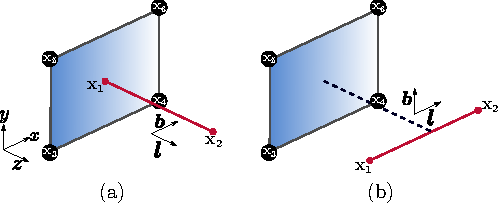
\includegraphics[width=0.8\linewidth]{test_gauss_quad.pdf}
    \caption[Test cases for comparing numeric v.s. analytic tractions using an edge dislocation near a surface.]{Simple test cases for an edge segment and surface element perpendicular (a) and parallel (b). The perpendicular dislocation is centered at the midpoint of the surface element, node $\mathbf{x_1}$ is separated by a perpendicular distance $\mathbf{x_1}^z$ to prevent the dislocation from intersecting the surface. On the right, the parallel dislocation runs along the $x$-axis at half the height of the surface element. The nodes of each dislocation line segment are kept at a perpendicular distance of at least one core radius away from the surface element.}
    \label{f:gauss_quad_test}
\end{figure}

The symmetry of these simple test cases benefits the accuracy of the numerical solutions because the stress fields exhibit symmetries about the dislocation line. If under ideal conditions for error cancellation, it can be proven that the numerical method is inferior to the analytic one, it can be more effectively argued that the analytic one should always be used instead.

\citet{analytic_tractions} found the analytic solution is approximately 10 times more computationally expensive than its numerical counterpart for 1 quadrature point, our findings agree with this result but the implications for a whole simulation are favourable (see \cref{ss:paperResults}).

One serious disadvantage of the analytic tractions is that the implementation of the analytic solution is also much more involved and full of snags. One issue is the calculation of the $y$-coordinate in the local coordinate frame as shown in \cref{f:force_lin_rect} and \cref{eq:problem}. If $\vec{l} \perp \vec{n}$, we get a singularity. As mentioned in \cite{analytic_tractions}, an easy fix is to rotate the line segment. We do this about its midpoint and around the $\vec{l} \times \vec{n}$ axis in both clockwise and anticlockwise directions. We use the mean of the values as the answer for $\theta = 0$. An example of what this rotation looks like in terms of the forces on a surface element can be seen in \cref{f:rotate} (avoiding the singularity at $\theta = 0$).
\begin{figure}
    \centering
    \subfloat[]{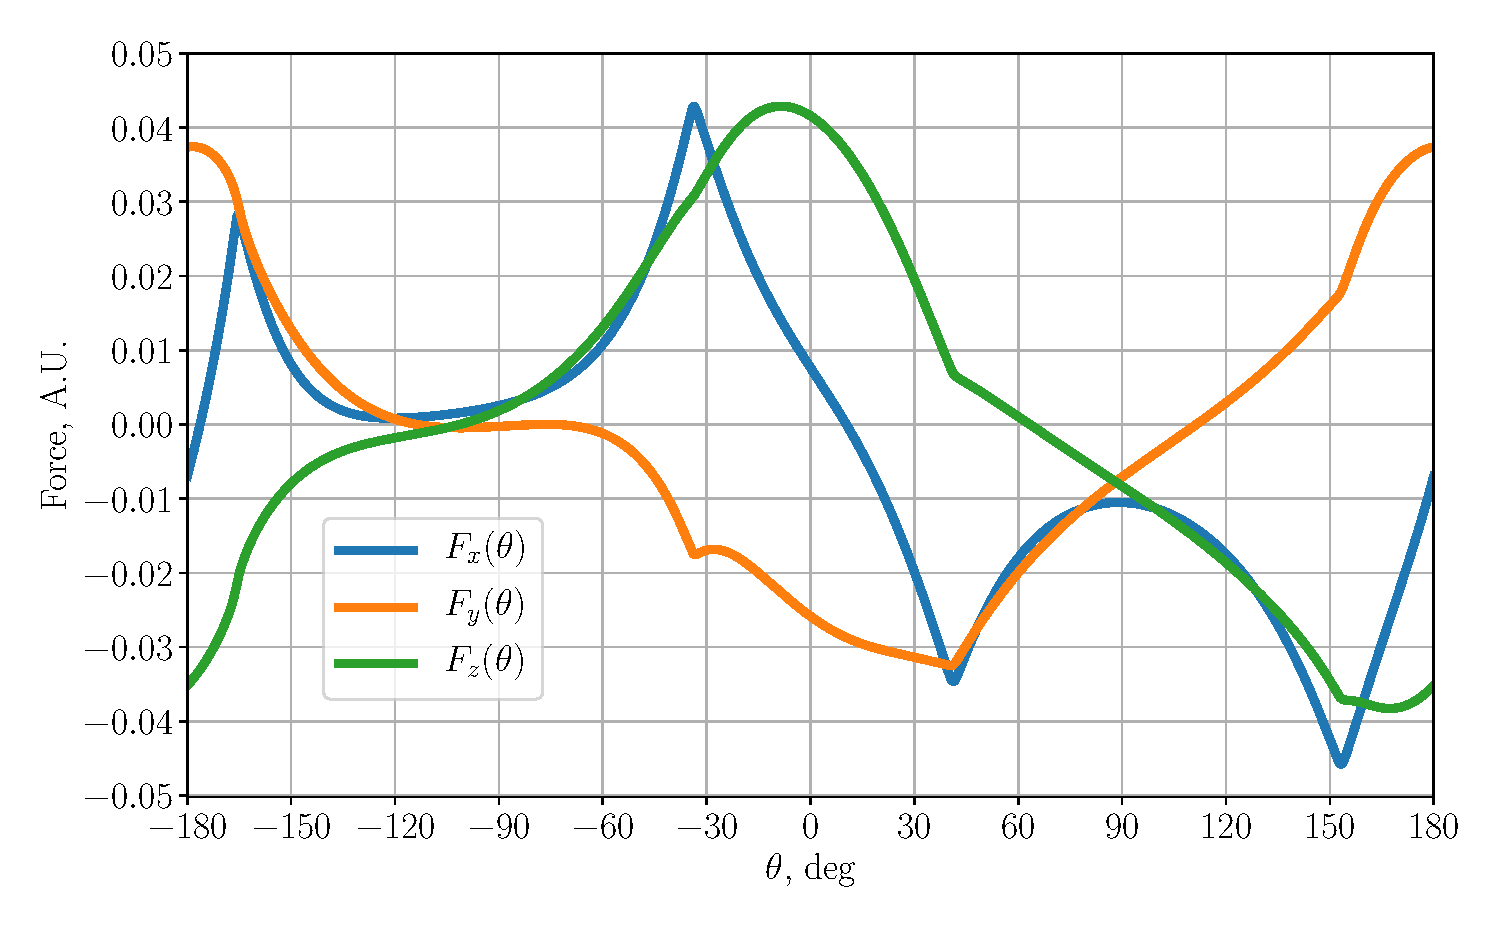
\includegraphics[width=0.45\linewidth]{ftot_rotation_lin_rect.pdf}}
    ~
    \subfloat[]{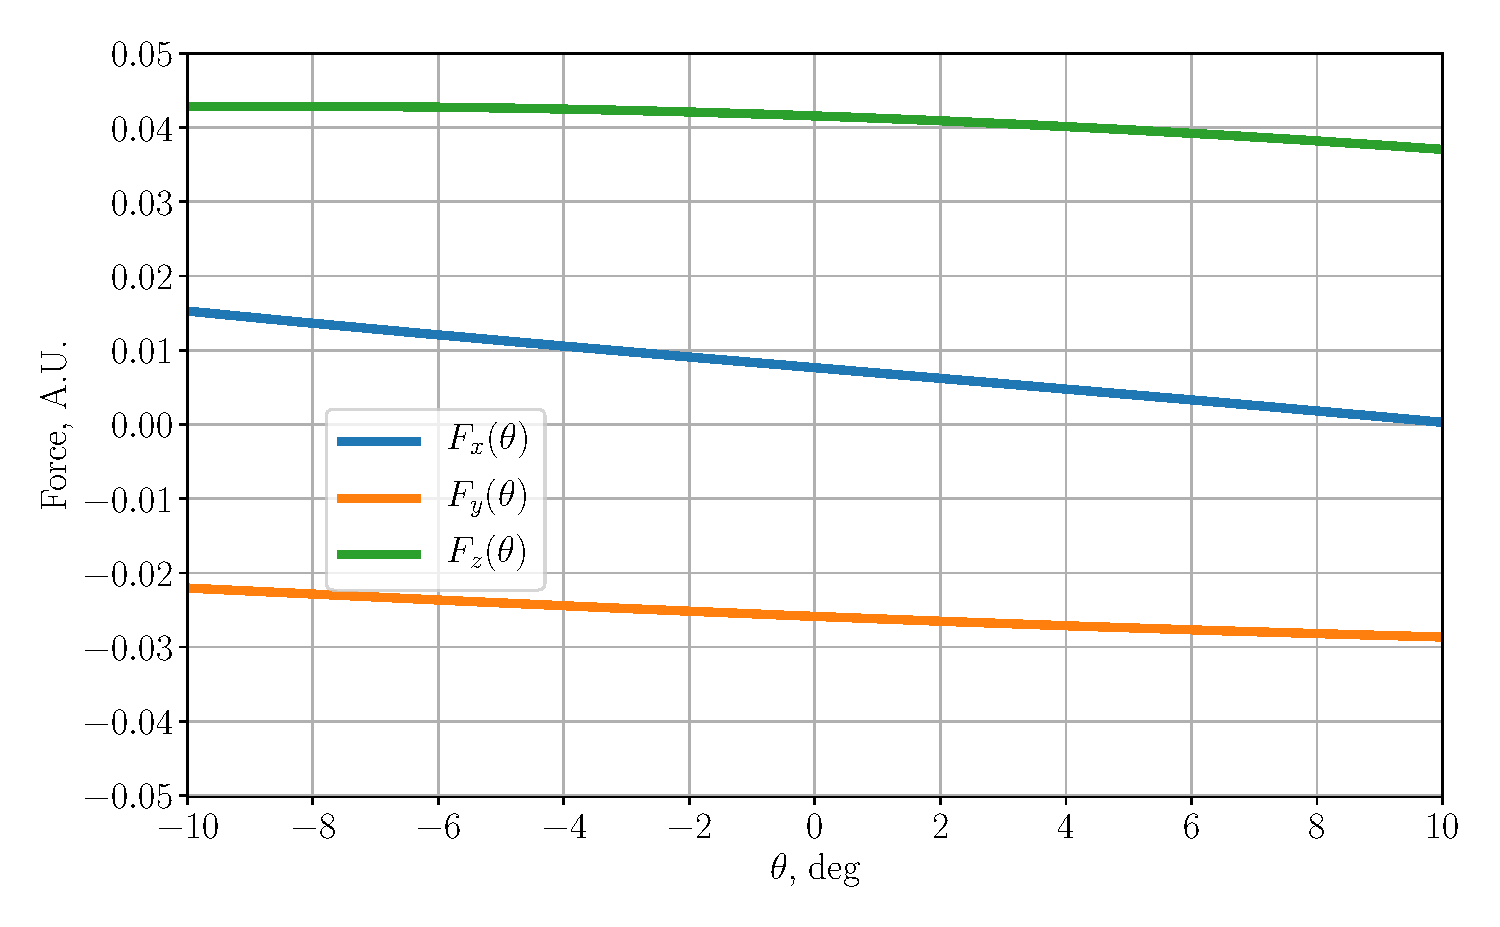
\includegraphics[width=0.45\linewidth]{ftot_rotation_lin_rect_zoom.pdf}}
    % \includegraphics[width=0.8\linewidth]{ftot_rotation_lin_rect_inlaid.pdf}
    \caption[Sample analytical forces on an element as a function of angle between surface and segment.]{(a) Example of the components of the total force on a surface element (the force summed over all four FE nodes) as a dislocation segment parallel to the surface element ($\theta = 0$) is rotated about its midpoint around the axis defined by $\vec{l}\times\vec{n}$. (b) is zomms into $\pm 10 \deg$, the force is smooth but not necessarily antisymmetric about the neighbourhood of $\theta=0$.}
    \label{f:rotate}
\end{figure}
The specific shape of the curves will vary depending on the element-segment configuration, but is smooth and well-behaved about singularity. For our purposes, we use a total of 8 perturbations of $1\deg$ each (4 clockwise and 4 anti-clockwise). We found this worked well, but can be changed if desired.

However, under finite-precision arithmetic, the check for orthogonality is dependent on the length scales involved in the simulation. This is particularly important considering the aforementioned use of arctangents, hyperbolic arctangents, logarithms and the large number of recurrence relations. Causing unexpected and rampant error propagation and numerical blow up is not difficult to achieve. When it happens, finding the root cause can lead one on a wild goose chase that is best avoided and often leads to a single segment in a single step of a long simulation that is slightly too small compared to its distance to a surface element to which it is slightly too parallel. To avoid these rare but high impact scenarios, we created a heuristic that dictates how strict the tolerance should be in order for the code to consider a segment to be parallel,
%
\begin{align}
    \lvert\vec{l}\cdot\vec{n}\rvert \lesssim \dfrac{\max\left(\lvert\vec{R}\cdot\vec{n}\rvert\right)}{10^8}\,.
\end{align}
%
In our case the numerator on the RHS is simply the FEM domain's largest dimension. $10^8$ is used instead of actual machine precision $\sim10^{15}$ because the seed functions and large number of recurrence relations of the solution propagate errors if the value of $\vec{l} \cdot \vec{n}$ is too close to zero. Ironically, tolerances which are too large can cause the perturbations to rotate the dislocation segment closer to the singularity, producing erroneous results. Larger than necessary tolerances can also slow down the calculation by detecting dislocations that are far enough from the special case that they can be treated like non-parallel segments. This heuristic is a good general purpose rule that keeps the tolerance in a goldilocks zone.

Another issue with the rotation is that one does not want a dislocation segment to intersect the surface when it is being rotated. Naively one would calculate the maximum rotational angle, $\theta_{\textrm{max}}$, to be,
%
\begin{align}
    \theta_{\textrm{max}} & = \arctan\left(\dfrac{2 d}{\left\lvert\mathbf{x_2} - \mathbf{x_1}\right\rvert}\right)\,.
\end{align}
%
Where $d$ is the minimum orthogonal distance from the dislocation to the surface element i.e. the collision distance---which in our case is a function of the dislocation core radius---and $\mathbf{x_1},\,\mathbf{x_2}$ are the dislocation segment node coordinates---whose maximum and minimum lengths are also functions of the dislocation core radius. However, $\theta_\textrm{max}$ might be too small in cases where the segment length is too small compared to the distance to a surface element, or when the segment length is much greater than $d$. Fine-tuning the angle is a task that involves knowing the minimum collision distance, minimum segment length, dislocation core radius, and the compiler's implementation of mathematical functions. Given the rarity of such cases and their comparatively low impact, we chose our $1\deg$ perturbation such that we safely avoid this problem while keeping within the bounds of the non-singular model.

Furthermore, the chirality and self-consistency of the FE nodes must be accounted for such that they are in the proper order regardless of the element face they belong to. Here we use 8-node linear hexahedral (brick) elements. The node ordering for the various surfaces is that for which the calculated normals point out from the the domain, this is dependant on the specific FE mesh implementation.

The total force on a given node must include the force contributions from every element in which said node appears, see \cref{f:shared_node}.
\begin{figure}
    \centering
    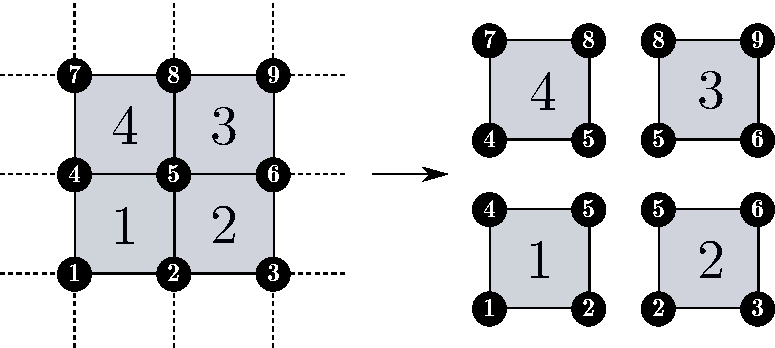
\includegraphics[width=\linewidth]{lrse_thread_map.pdf}
    \caption[FE nodes are shared between surface elements.]{FE nodes are shared by either 4 element faces or 3 if it is a corner node. The total force on a given node is the summation of the force contributions from each element it belongs to.}
    \label{f:shared_node}
\end{figure}
The specifics of the mapping depend on the global FE node numbering. Using \cref{f:shared_node} as our reference labels for elements and nodes, $e$ and $n$ respectively, we can give a concrete example of how this is done by defining,
\begin{subequations}
    \begin{align}
        \vec{x_{e,n}} & \equiv	\begin{bmatrix}
            x_{e,n} & y_{e,n} & z_{e,n}
        \end{bmatrix}^{\mathsf{T}}, \quad
        \vec{x_{n}} \equiv	\begin{bmatrix}
            x_{n} & y_{n} & z_{n}
        \end{bmatrix}^{\mathsf{T}}            \\
        \begin{split}
            \mtx{N_{L}} &=	\begin{bmatrix}
                l_{1,1} & l_{1,2} & l_{1,4} & l_{1,5} \\
                l_{2,2} & l_{2,3} & l_{2,5} & l_{2,6} \\
                l_{3,5} & l_{3,6} & l_{3,8} & l_{3,9} \\
                l_{4,4} & l_{4,5} & l_{4,7} & l_{4,8} \\
            \end{bmatrix}
        \end{split}
        , \quad
        \vec{\gamma} =   \begin{bmatrix}
            l_1    \\
            l_2    \\
            \vdots \\
            l_9
        \end{bmatrix}                          \\
        \begin{split}
            \mtx{F_{e}} &=	\begin{bmatrix}
                \vec{x_{1,1}} & \vec{x_{1,2}} & \vec{x_{1,4}} & \vec{x_{1,5}} \\
                \vec{x_{2,2}} & \vec{x_{2,3}} & \vec{x_{2,5}} & \vec{x_{2,6}} \\
                \vec{x_{3,5}} & \vec{x_{3,6}} & \vec{x_{3,8}} & \vec{x_{3,9}} \\
                \vec{x_{4,4}} & \vec{x_{4,5}} & \vec{x_{4,7}} & \vec{x_{4,8}} \\
            \end{bmatrix}
        \end{split}
        ,\quad
        \vec{\tilde{F}} = 	\begin{bmatrix}
            \vec{x_{1}} \\
            \vec{x_{2}} \\
            \vdots      \\
            \vec{x_{9}}
        \end{bmatrix}\,.\label{eq:force_imp}
    \end{align}
\end{subequations}
Where $\vec{x_{e,n}}$ is a $3\times1$ column vector corresponding to the $(x\,,y\,,z)$ dislocation induced forces on node, $n$, on the surface element, $e$. There are four of these per rectangular surface element, where a given node, $n$, can appear in multiple surface elements (e.g. node 5 in \cref{f:shared_node} is shared by all 4 surface elements), all of which independently contribute to the total force on said node. $\vec{x_n}$ is a $3\times1$ column vector corresponding to the total $(x\,,y\,,z)$ dislocation induced forces on node $n$. These are used to shorten the definition of \cref{eq:force_imp} and are not explicitly defined in the implementation, rather they give the force matrices $\mtx{F_{e}}$ and $\vec{\tilde{F}}$ a specific row order. $\mtx{N_{L}}$ is crucial for the correct implementation of this analytical solution in traditional FE codes. It is the $E\times4$ matrix corresponding to the global label of each node in a given surface element. Each row of the matrix represents a surface element and each column represents a node in the surface element. We cannot na\"ively add the columns together as that would give the total force acting on the element as a whole, not each FE node individually. We chose to arrange the columns in accordance to \cref{f:force_lin_rect} as it makes it easier to implement the solution, but the only thing that matters is that the basis vectors $\vec{n},\,\vec{p},\,\vec{q}$ are calculated appropriately. $\vec{\gamma}$ is the vector with the FE node labels, which makes mapping force to node possible. $\mtx{F_{e}}$ is the $3E \times 4$ matrix where the forces acting on each of the four nodes (column) in a particular surface element (each element corresponds to three consecutive rows because there are three dimensions) are stored. $\vec{\tilde{F}}$ is the $3N\times1$ column vector where the total forces on each node are stored (each node has three rows because there are three dimensions). This is easily generalisable to $E$ elements and $N$ nodes.

\Cref{a:tot_force} illustrates how the total force on each node is obtained. However, our implementation does not strictly follow it because we memoise a generalised version of $\vec{L}$ upon simulation initialisation instead of finding one at every iteration, reducing computational time but requiring us to account for nodes without traction boundary conditions. Our indexing also starts at 1, but zero indexing makes the algorithm easier to follow.
\begin{algorithm}
    \caption[Calculating total force on a node using analytic tractions.]{Assuming $ \vec{\tilde{F}} $ is arranged the same way as $ \vec{\gamma} $ and indexing starts at 0.}
    \begin{algorithmic}[1]
        \label{a:tot_force}
        \State\Comment{Loop through the array containing the node labels of the relevant surface nodes.}
        \For{$ i = 0;\, i < \rvar{length}(\vec{\gamma});\, i++$}					\State\Comment{Save the global node label for the current iteration.}
        \State $ n \gets \vec{\gamma}[i] $
        \State\Comment{Use the node label to find a vector, $\vec{L}$, with the linearised indices in $\mtx{N_{L}}$ where node $n$ appears as part of a surface element whose tractions we are calculating.}
        \State $ \vec{L} \gets \rvar{find}(\mtx{N_{L}} == n) $
        \State\Comment{Loop over coordinates.}
        \For{$ k = 0;\, k < 3;\, k++ $}
        \State\Comment{Use global node label vector to index the force array from the analytical force calculation. Multiplied by 3 because there are three coordinates per node. We sum the forces from the analytical calculation because the same global node can be part of multiple surface elements. We add $ k $ because the $ x,~y,~z $ coordinates are consecutively stored in $ \mtx{F_{e}} $.}
        \State $ \vec{\tilde{F}}[3n + k] \gets \vec{\tilde{F}}[3n + k] + \sum\mtx{F_{e}}[3\vec{L} + k]  $
        \EndFor
        \EndFor
    \end{algorithmic}
\end{algorithm}

The resulting force vector is then used in \cref{eq:thatbc} to calculate $\tns{\hat{\sigma}}$, since $\tilde{\vec{T}} \equiv \tilde{\vec{F}}$. \Cref{f:headvstractionfem} shows the simple system we used to compare the image stresses calculated by our FE solver using numeric tractions v.s. analytic tractions v.s. infinite-domain, singular image stresses in \cref{eq:imageStressAnalyticEdge1,eq:imageStressAnalyticEdge2,eq:imageStressAnalyticScrew}. The three test cases are: two edge dislocations and one screw, all of which have line direction $\vec{l} = [0\, 0\, 1]$. The Burgers vectors for the different scenarios are $\vec{b}_\textrm{e1} \equiv \vec{b} = [1\, 0\, 0]$, $\vec{b}_\textrm{e2} \equiv \vec{b} = [0\, 1\, 0]$, as defined in \cite{head1953edge}; and $\vec{b}_\textrm{s} \equiv \vec{b} = \vec{l} = [0\, 0\, 1] $, as defined in \cite[p.~59,~64]{hirth1983theory}.

The units in all our examples are normalised to lattice parameter, $a$ is the dislocation core radius for the non-singular formulation discussed in \cite{a_non-singular_continuum_theory_of_dislocations}, and $b \equiv \lVert \vec{b} \rVert$.

\begin{figure}
    \centering
    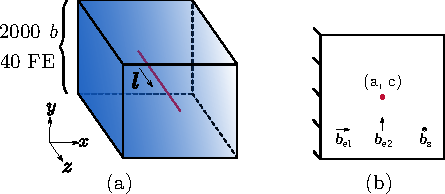
\includegraphics[width=0.8\linewidth]{head_vs_fe_tractions_setup_diagram.pdf}
    \caption[Set up comparing infinite-domain, singular solutions of stress fields to those obtained via a non-singular formulation with analytic and numeric tractions coupled to FEM.]{Dislocation parallel to a surface described by the line $x = 0$, where the $(x,\,y)$ dislocation coordinates are $(a,\,c)$ and the dislocation line going in the positive $z$-direction. (a) describes the box we used for our comparison, a  $40 \times 40 \times 40$ element cubic box with side lengths equal to $2000$ with $\vec{T} = \bm{0}$, traction boundary conditions only on the nodes along $x = 0$, and $\vec{U} = \bm{0}$, displacement conditions everywhere else. (b) is the 2D view with the dislocation coordinates $(a,~c)$, as well as the two edge Burgers vectors in \cite{head1953edge}, $\vec{b}_\textrm{e1} \equiv \vec{b} = [1\, 0\, 0]$, $\vec{b}_\textrm{e2} \equiv \vec{b} = [0\, 1\, 0]$ and the screw Burgers vector $\vec{b}_\textrm{s} \equiv \vec{b} = \vec{l} = [0\, 0\, 1] $ in \cite[p.~59,~64]{hirth1983theory}.}
    \label{f:headvstractionfem}
\end{figure}

The slices we took for our contour plots in \cref{ss:paperResults} are on the middle plane of the domain at $z = 1000$.

We also ran a very simple simulation comparing the results between using analytic tractions as opposed to numeric ones. Finding a simple yet clear case of tractions producing catastrophically wrong behaviours can be difficult. Large differences in image forces are relatively rare and other factors often dominate. Such factors include the core radius---which affects the dislocation line tension and therefore works against the deformation of a dislocation line---mobility law and mobility parameters used, external loading, etc.

However, we found a simple and realistic configuration that is close to the setup in the infinite domain examples. The differences between those comparisons and the simulation are described in \cref{t:simulation_params}. We use a mobility law developed in-house by B. Bromage \cite{bromage2018calculating}, that corrects common issues found in other laws. We also rotate the domain such that the $[1\, 1\, 1]$ and $[1\, \overline{1}\, 0]$ crystallographic directions respectively correspond to the simulation's $x$ and $y$-directions, for this we use the same rotation technique as \cite{YU2018}. The dislocation was allowed to move under no external loads or displacements, with $\vec{T} = \bm{0}$ boundary conditions only on the $yz$-plane and $\vec{U} = \bm{0}$ everywhere else.
\begin{table}
    \centering
    \caption[Numeric v.s. analytic tractions. Unloaded simulation comparison.]{Parameters for our simulation. Where $\mtx{R}$ is a rotation matrix such that the $\vec{x},\, \vec{y},\, \vec{z}$ basis vectors of our simulation correspond to the $\vec{b},\, \vec{n},\, \vec{l}$ crystallographic directions, i.e. $\mtx{R} \vec{x} = \vec{b}$. Everything else was kept just as the previous comparisons. All values are in units of lattice parameters.}
    \label{t:simulation_params}
    \begin{tabular}{ll}
        \toprule
        Parameter          & Value                                           \\
        \midrule
        Crystal Structure  & BCC                                             \\
        $\vec{b}$          & $[1\, 1\, 1]$                                   \\
        $\vec{n}$          & $[1\, \overline{1}\, 0]$                        \\
        $\vec{l}$          & $[1\, 1\, \overline{2}]$                        \\
        $b$                & $\sqrt{3}/2$                                    \\
        $a$                & $5\, $                                          \\
        Grid Size          & $(20,\, 20,\, 20)$                              \\
        Domain Size        & $(2000,\, 2000,\, 2000)\, $                     \\
        Lattice size       & $3.18\times 10^{-4}~\mu\text{m}$                \\
        $(x_{0},\, y_{0})$ & $(62.5,\, 1000)\, $                             \\
        Min segment length & $50\, $                                         \\
        Max segment length & $125\, $                                        \\
        $\mtx{R}$          & $[\hat{\vec{b}}~ \hat{\vec{n}}~ \hat{\vec{l}}]$ \\
        \bottomrule
    \end{tabular}
\end{table}

\subsection{Results and Discussion}\label{ss:paperResults}

\Cref{f:rel_err_perp_edge} shows that even for dislocations only one dislocation core radius ($5$) away from the surface element, the force can be obtained, up to numerical precision, with 1000 Gauss quadrature points $Q$ for all segment lengths tested. It also shows a very peculiar issue Gauss quadrature has when computing integrals of rational functions when the Gauss nodes are close poles/maximal values. This undesirable behaviour is observed in the case where $Q = 11$. Where the highest weighted Gauss node is closest to the point where $1/R_{a}$ is maximal, resulting in lower accuracy when compared to $Q = 2, 10$ in \cref{f:rel_err_perp_edge} (a) and (b).
\begin{figure}
    \centering
    \subfloat[Segment starts a single dislocation core radius away.]
    {
        {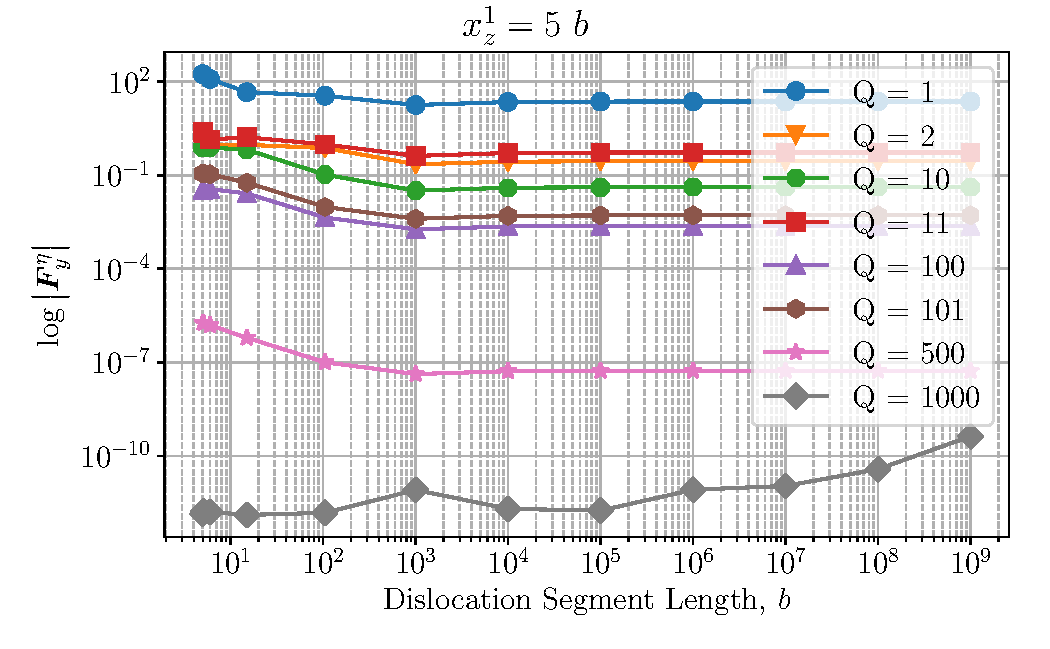
\includegraphics[trim={0.5cm 0.55cm 0.65cm 0.1cm},clip,width=0.475\linewidth]{perp_e_xz=5.pdf}}
    }
    ~
    \subfloat[Segment starts 3 dislocation core radii away.]
    {
        {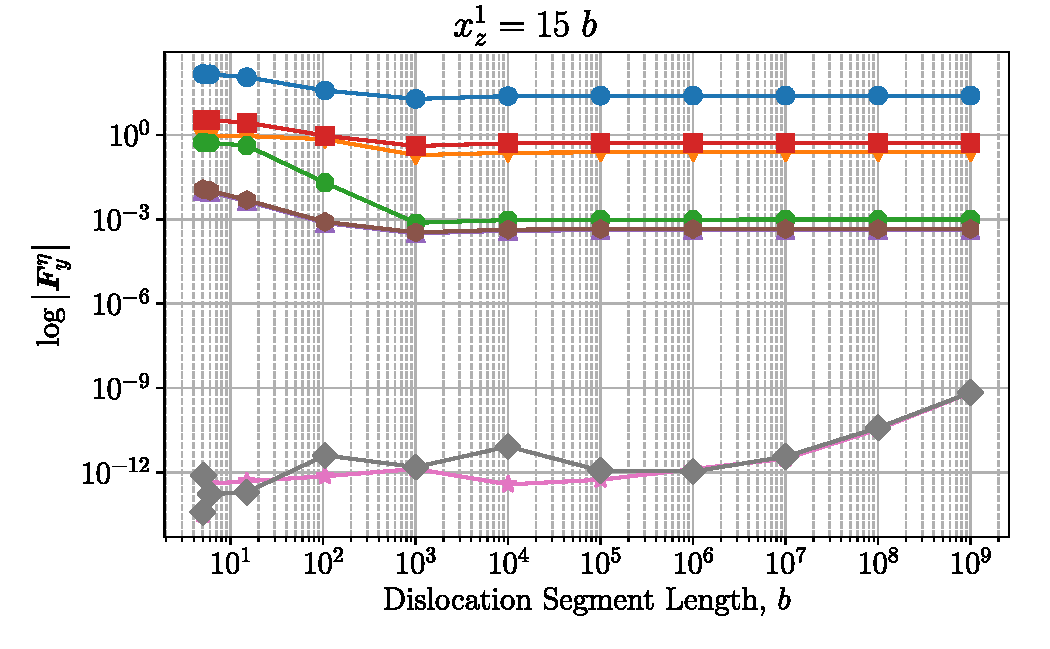
\includegraphics[trim={0.5cm 0.55cm 0.65cm 0.1cm},clip,width=0.475\linewidth]{perp_e_xz=15_leg.pdf}}
    }

    \subfloat[Segment starts 201 dislocation core radii away.]
    {
        {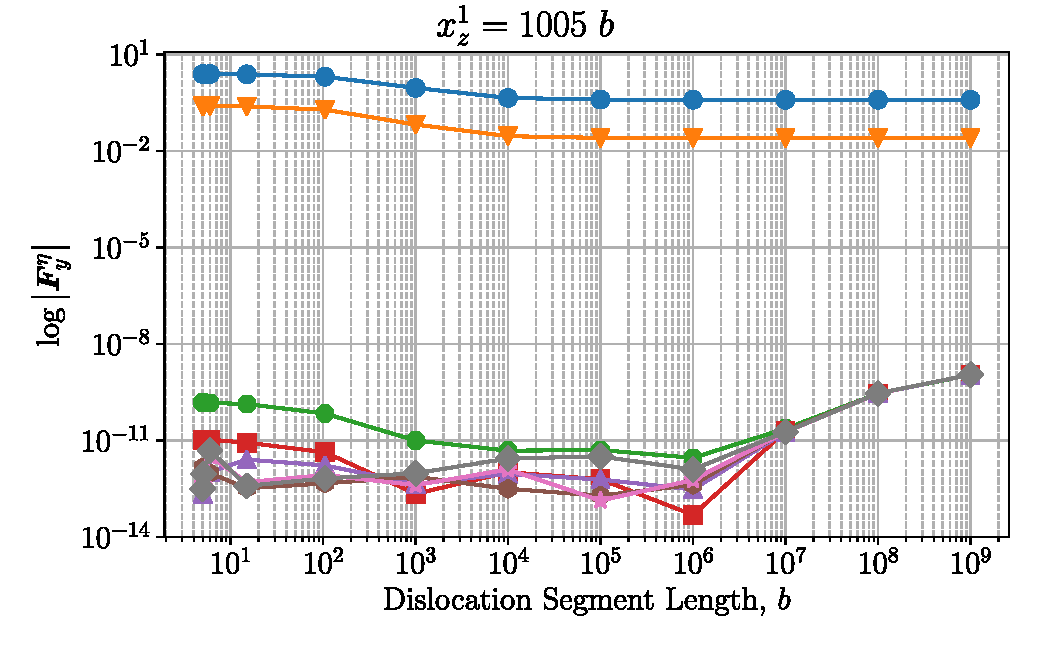
\includegraphics[trim={0.5cm 0.55cm 0.65cm 0.1cm},clip,width=0.475\linewidth]{perp_e_xz=1005_leg.pdf}}
    }
    ~
    \subfloat[Segment starts 20001 dislocation core radii away.]
    {
        {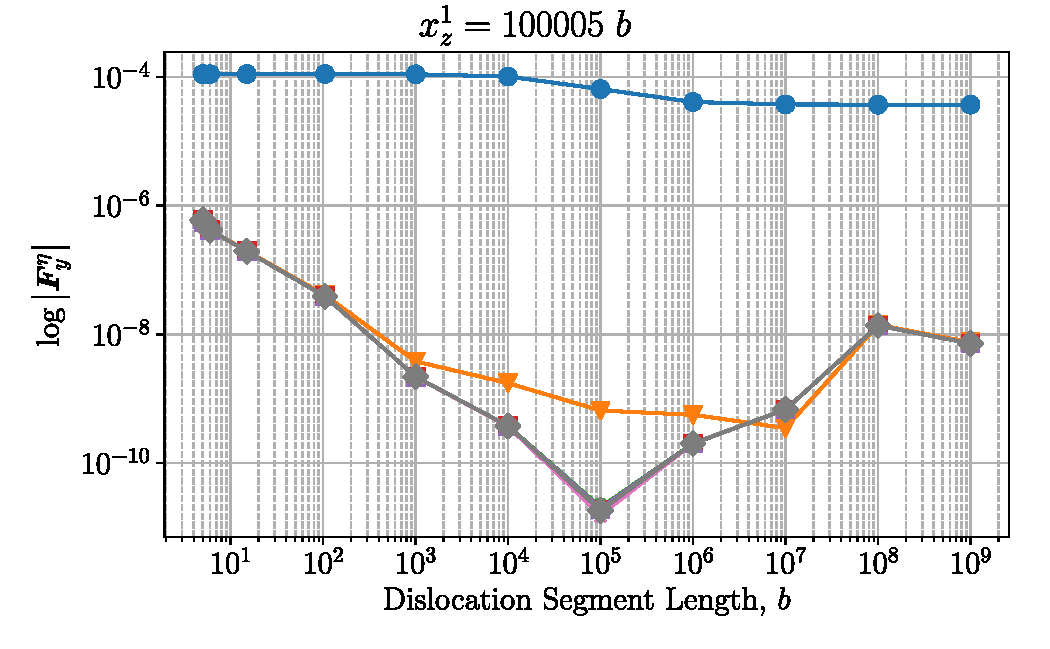
\includegraphics[trim={0.5cm 0.55cm 0.65cm 0.1cm},clip,width=0.47\linewidth]{perp_e_xz=100005_leg.pdf}}
    }
    \caption[Relative error for an edge dislocation perpendicular to a surface element.]{Log-log plot of the relative error as a function of dislocation segment length for a perpendicular edge dislocation (\cref{f:gauss_quad_test}a). $x^{1}_{z}$ is the $z$-coordinate of node $\mathbf{x_1}$. $\vec{b} = [1\, 0\, 0]$, line direction, $\vec{l} = [0\, 0\, 1]$, and dislocation core radius, $a = 5$, the surface element's normal and size are, $\vec{n} = [0\, 0\, 1]$, $L = 1000$, respectively. $Q$ is the number of quadrature points per dimension.}
    \label{f:rel_err_perp_edge}
\end{figure}
It is worth noting however that the relative errors for small numbers of quadrature points don't really start decreasing until relatively large distances. And when close to a surface, these can be quite large even under highly symmetric circumstances.

The limitations become even more evident when the dislocation line segment is parallel to a surface element. In \cref{f:rel_err_par_edge}, we observe the relative errors are quite large when close to the surface. At distances larger than $10^4\, $, loss of significance causes the relative errors to converge at $\sim 1$ which is expected as two finite precision floating point numbers get closer to zero. Of particular note is how large the relative errors are even at $100$ lattice units away from the surface, even for large numbers of quadrature points. This figure backs up the earlier point regarding Gauss nodes close to maximal values of rational functions. It can be shocking to see that as $Q = 2$ performs significantly better than $Q = 10, 11, 100, 100$ at distances from the surface as having nodes near the maximal values is a large source of error. Consequently, different configurations have different optimal numbers of points. The numerical instability of this method, which when coupled to the chaotic nature of dislocation dynamics and stiffness of the equations of motion, can lead to large deviations between simulations.
\begin{figure}
    \centering
    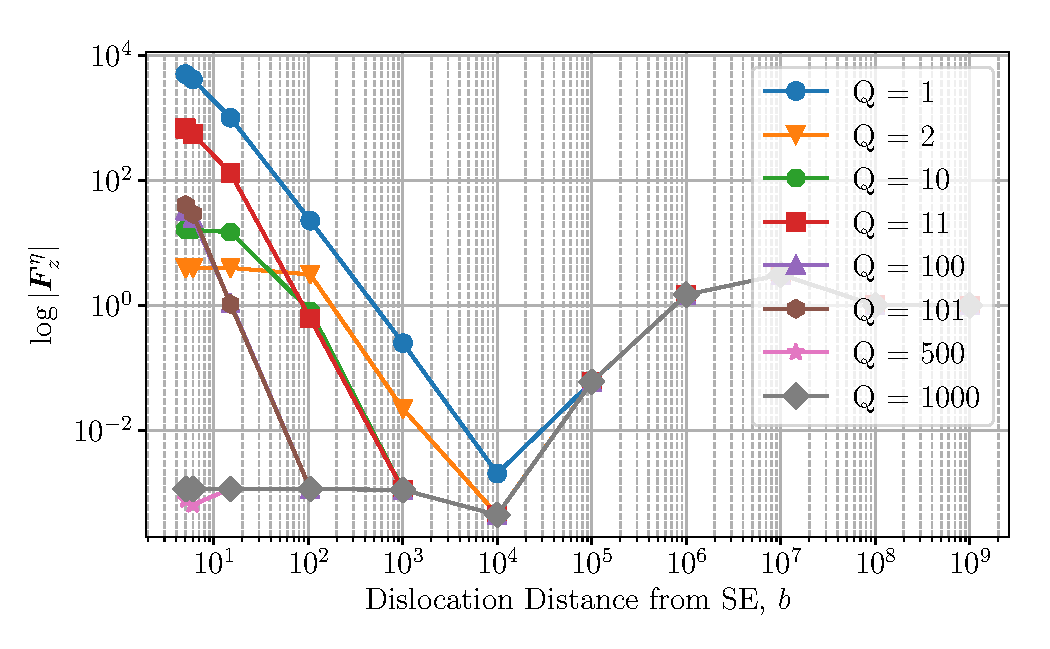
\includegraphics[width=0.8\linewidth]{par_e_z.pdf}
    \caption[Relative error for an edge dislocation parallel to a surface element.]{Log-log plot of the relative error as a function of distance from the surface element for a parallel edge dislocation (\cref{f:gauss_quad_test}b). Burgers vector, $\vec{b} = [0\, 1\, 0]$, line direction, $\vec{l} = [1\, 0\, 0]$, dislocation core and surface element parameters are the same as \cref{f:rel_err_perp_edge}. The dislocation length is fixed to $10^{6},\, x\in\left[-0.5\times10^{6},\, 0.5\times10^{6} \right]$ and bisects the surface element along the $[1\, 0\, 0]$ direction. The whole dislocation was segmented into $10^4$ pieces of length $100$ to prevent the dislocation from intersecting the surface element when they were rotated to avoid the singularity. The relative error at large distances ($>10^6\, $) converges to one due to loss of significance.}
    \label{f:rel_err_par_edge}
\end{figure}

From \cref{f:rel_err_perp_edge,f:rel_err_par_edge} one might be tempted to say that for a segment parallel to a surface, Gauss quadrature performs far worse than for a perpendicular one. However there is a further wrinkle in this problem: symmetry. To exemplify this we plot the relevant components of the stress tensor for the arrangement found in \cref{f:gauss_quad_test}(a) in \cref{sf:xzeperp,sf:yzeperp,sf:zzeperp}. The $\sigma_{xz}$ and $\sigma_{zz}$ components are antisymmetric about the centre of the element. If we use Gauss quadrature on them, we sample equivalent but oppositely valued points that are equally weighted, thus the sum vanishes and therefore do not contribute to \cref{f:rel_err_perp_edge}. However, $\sigma_{yz}$ does not vanish, but can be accurately integrated with sufficiently large $Q$. If we were to move the dislocation off-centre such that these symmetries are broken, the errors would increase.

We also plot the relevant stresses for the arrangement described by \cref{f:gauss_quad_test}(b) in \cref{sf:xzepar,sf:yzepar,sf:zzepar}. From \cref{sf:xzepar} and \cref{sf:yzepar}, it is immediately apparent why gauss quadrature fails so spectacularly in \cref{f:rel_err_par_edge}. At low numbers of quadrature points, it fails to appropriately sample the rapidly changing value of $\tilde{\sigma}_{xz}$ at both ends of the dislocation, as well those in the neighbourhood of the dislocation in $\tilde{\sigma}_{yz}$. Moreover, the further away the quadrature points are from the midpoint of the domain, the lower their relative weighting. So even with a relatively large number of them, there can still be large errors. Which is a particularly egregious problem in \cref{sf:yzepar}, and explains why such a large number of quadrature points is required to accurately compute the integral.
\begin{figure}
    \centering
    \subfloat[\label{sf:xzeperp}]
    {
        {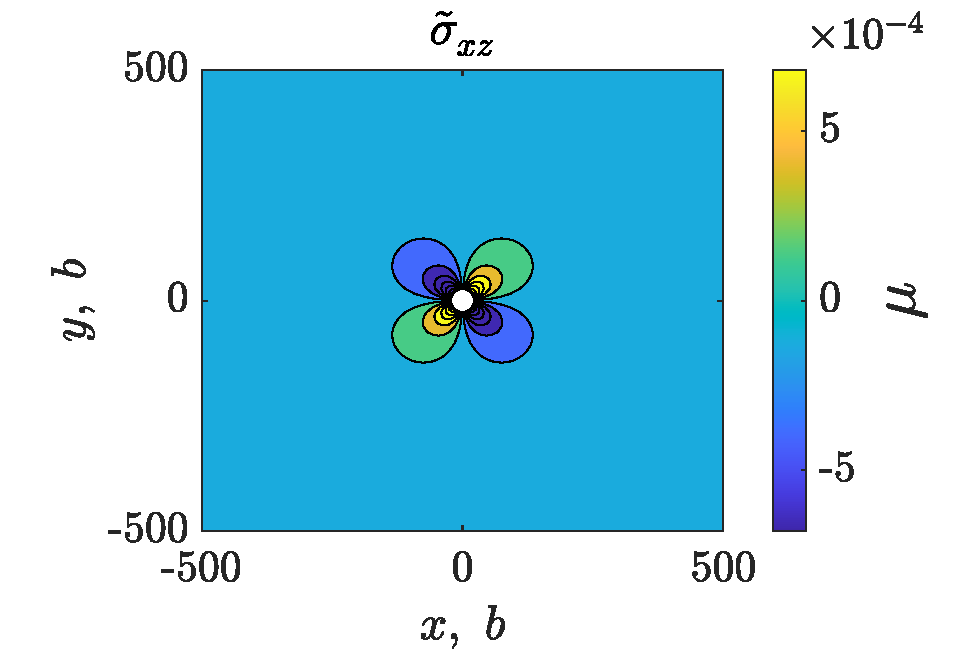
\includegraphics[trim={0.5cm 0cm 0cm 0cm},clip,width=0.3\linewidth]{sxzperpEdgeFiveb.pdf}}
    }
    ~
    \subfloat[\label{sf:yzeperp}]
    {
        {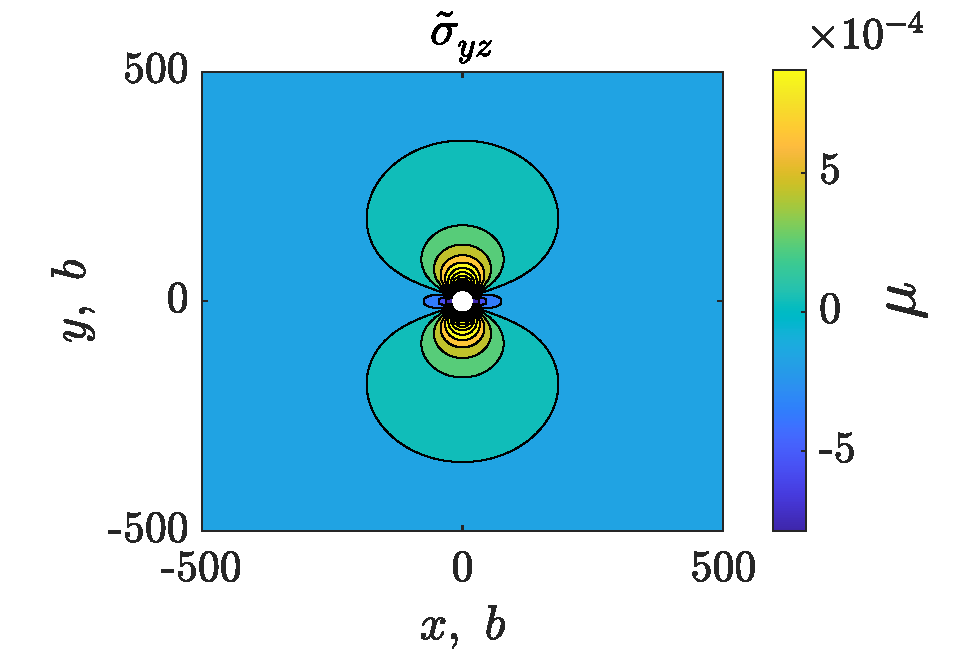
\includegraphics[trim={0.5cm 0cm 0cm 0cm},clip,width=0.3\linewidth]{syzperpEdgeFiveb.pdf}}
    }
    ~
    \subfloat[\label{sf:zzeperp}]
    {
        {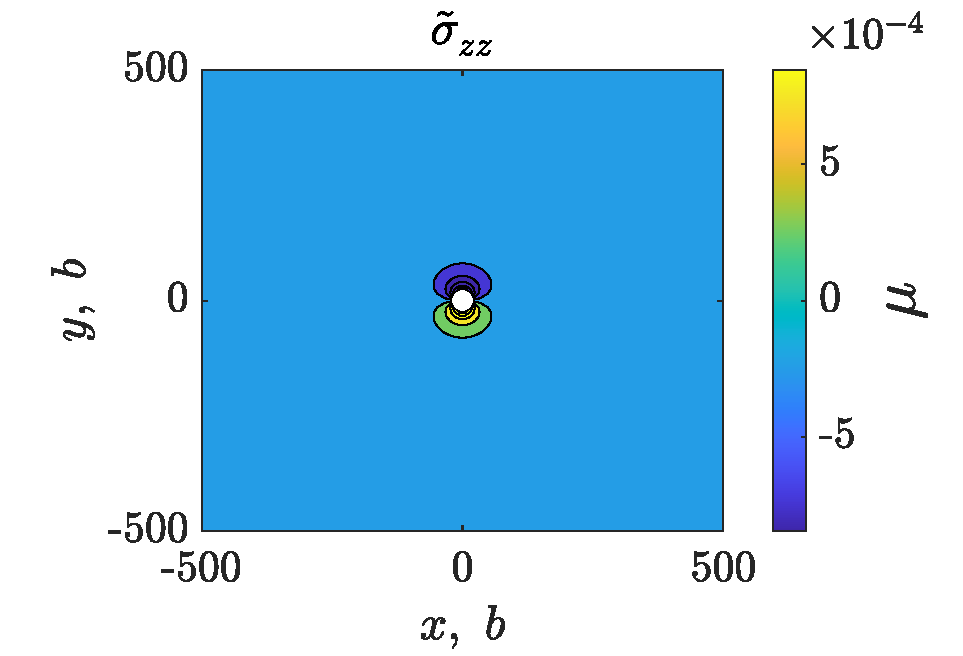
\includegraphics[trim={0.5cm 0cm 0cm 0cm},clip,width=0.3\linewidth]{szzperpEdgeFiveb.pdf}}
    }

    \subfloat[\label{sf:xzepar}]
    {
        {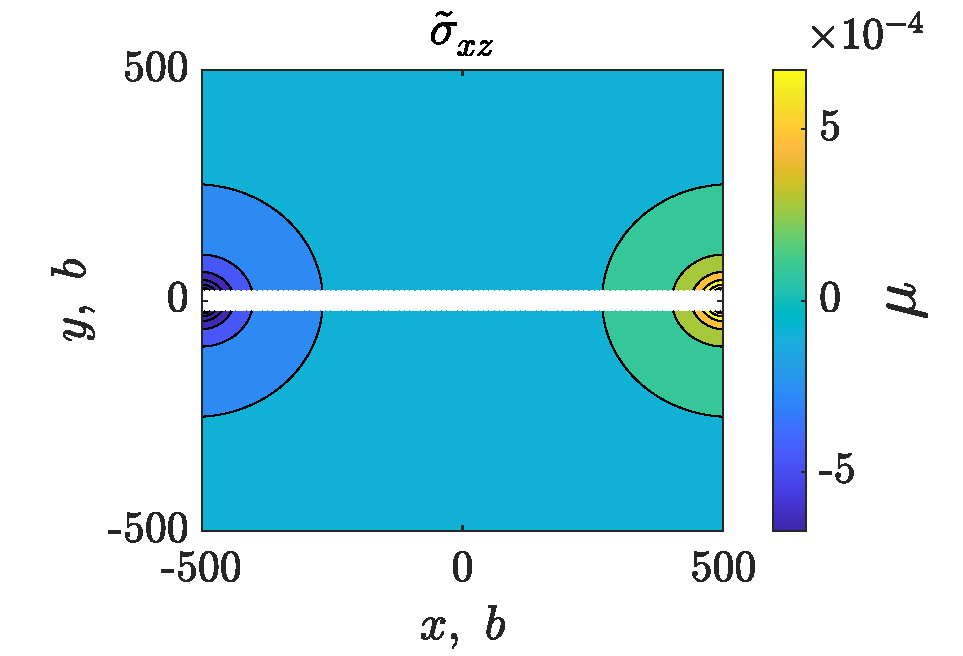
\includegraphics[trim={0.5cm 0cm 0cm 0cm},clip,width=0.3\linewidth]{sxzparEdgeFiveb.pdf}}
    }
    ~
    \subfloat[\label{sf:yzepar}]
    {
        {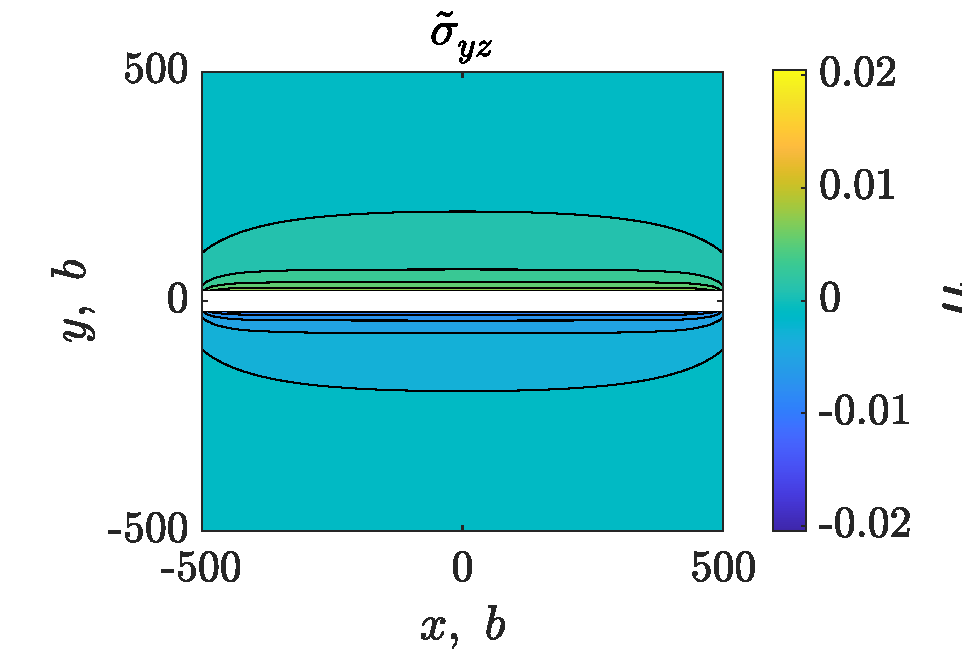
\includegraphics[trim={0.5cm 0cm 0cm 0cm},clip,width=0.3\linewidth]{syzparEdgeFiveb.pdf}}
    }
    ~
    \subfloat[\label{sf:zzepar}]
    {
        {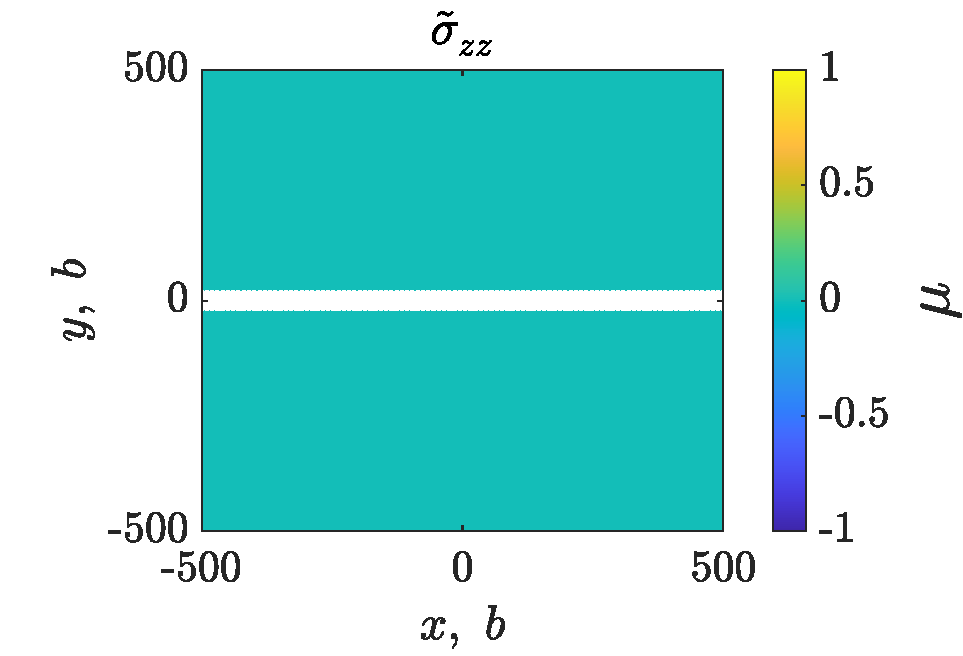
\includegraphics[trim={0.5cm 0cm 0cm 0cm},clip,width=0.3\linewidth]{szzparEdgeFiveb.pdf}}
    }
    \caption[Symmetry in stress fields leads more accurate numeric tractions.]{(a) to (c) show the real stress fields from a dislocation in the same configuration that yields the plots found in \cref{f:rel_err_perp_edge} as shown in \cref{f:gauss_quad_test}(a), where the closest node is a dislocation core radius away from the surface, $a = 5$. (e) to (f) does the same for the configuration that yields \cref{f:rel_err_par_edge} as shown in \cref{f:gauss_quad_test}(b), where the whole dislocation is a core radius away from the surface, $a = 5$. The white line or dot is the dislocation. Units are in terms of lattice parameters.}
    \label{f:sigma_edge_test_config}
\end{figure}

Despite these being artificially idealised examples that illustrate the failings of Gauss quadrature, other problematic scenarios commonly show up in simulations. These tend to worsen with smaller core radii $a$, fewer Gauss nodes, higher dislocation densities near surfaces, more permissive mobility functions, and coarser FE meshes. The $\mathcal{O}(1/R)$ decay rate of $\tns{\tilde{\sigma}}$ and chaotic nature of dislocation dynamics, means these errors may result in unwarranted topological changes that cascade as the simulation advances. This is particularly deleterious when doing simulations with higher dislocation densities and/or where a large number of dislocations are close to the surface, such as nanoindentation simulations.

\begin{figure}
    \centering
    \subfloat[%$\hat{\sigma}_{xx}$.
        \hspace{-0.8cm}\label{sf:sxxeperp}]
    {
        {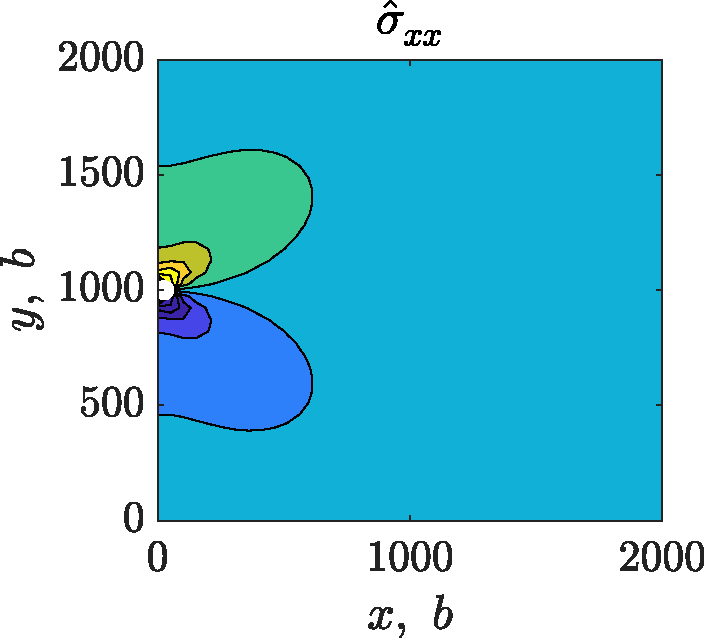
\includegraphics[width=0.25\linewidth]{sxxEperp_leg.pdf}}
    }~
    \subfloat[%$\hat{\sigma}^\textrm{A}_{xx}$.
        \hspace{-0.8cm}\label{sf:sxxAeperp}]
    {
        {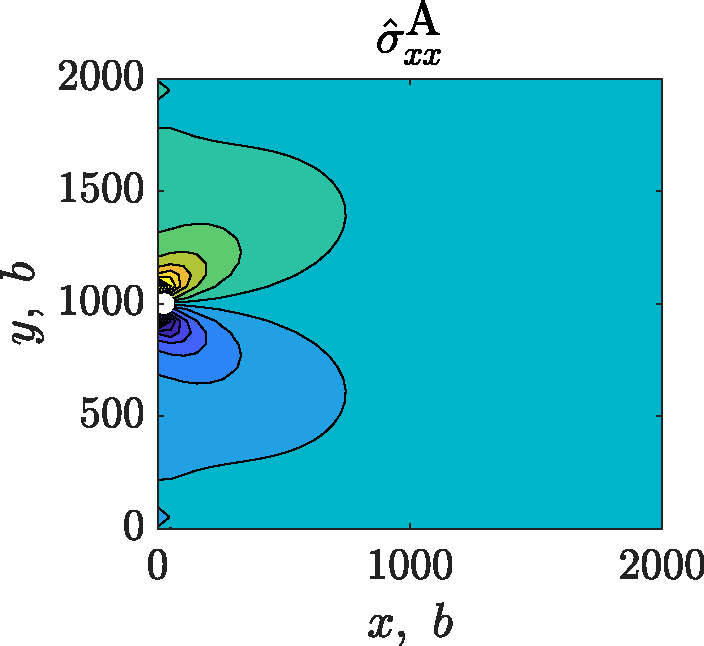
\includegraphics[width=0.25\linewidth]{sxxAEperp_leg.pdf}}
    }~
    \subfloat[%$\hat{\sigma}^\textrm{N}_{xx}$.
        \hspace{-0.8cm}\label{sf:sxxNeperp}]
    {
        {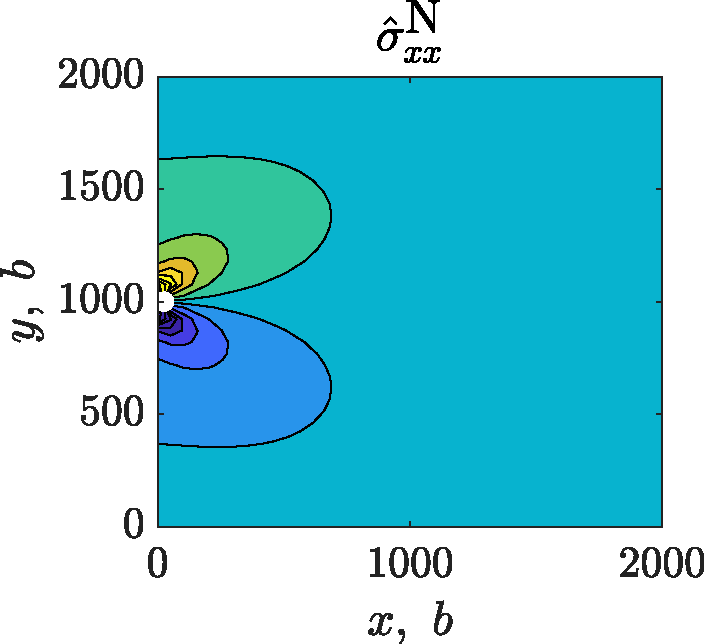
\includegraphics[width=0.25\linewidth]{sxxNEperp_leg.pdf}}
    }~
    \subfloat{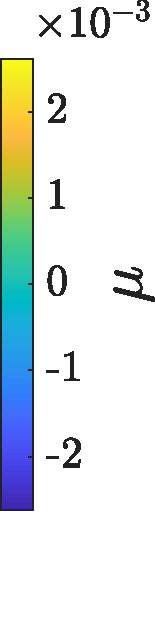
\includegraphics[height = 0.22\linewidth]{sxxNAEperp_leg.pdf}}

    \subfloat[%$\hat{\sigma}_{yy}$.
        \hspace{-0.8cm}\label{sf:syyeperp}]
    {
        {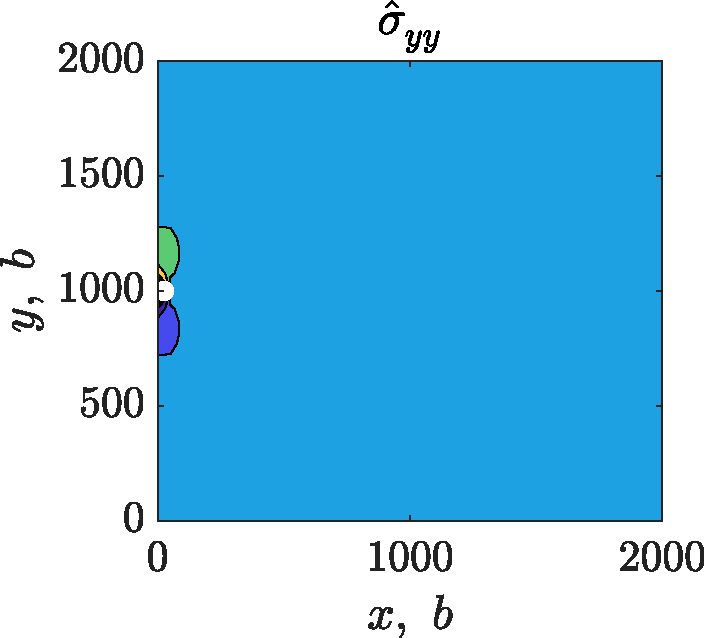
\includegraphics[width=0.25\linewidth]{syyEperp_leg.pdf}}
    }~
    \subfloat[%$\hat{\sigma}^\textrm{A}_{yy}$.
        \hspace{-0.8cm}\label{sf:syyAeperp}]
    {
        {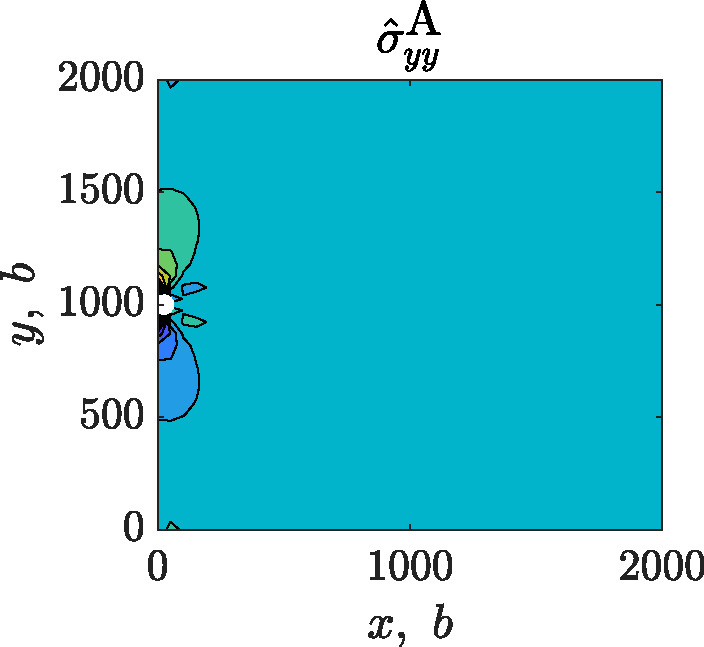
\includegraphics[width=0.25\linewidth]{syyAEperp_leg.pdf}}
    }~
    \subfloat[%$\hat{\sigma}^\textrm{N}_{yy}$.
        \hspace{-0.8cm}\label{sf:syyNeperp}]
    {
        {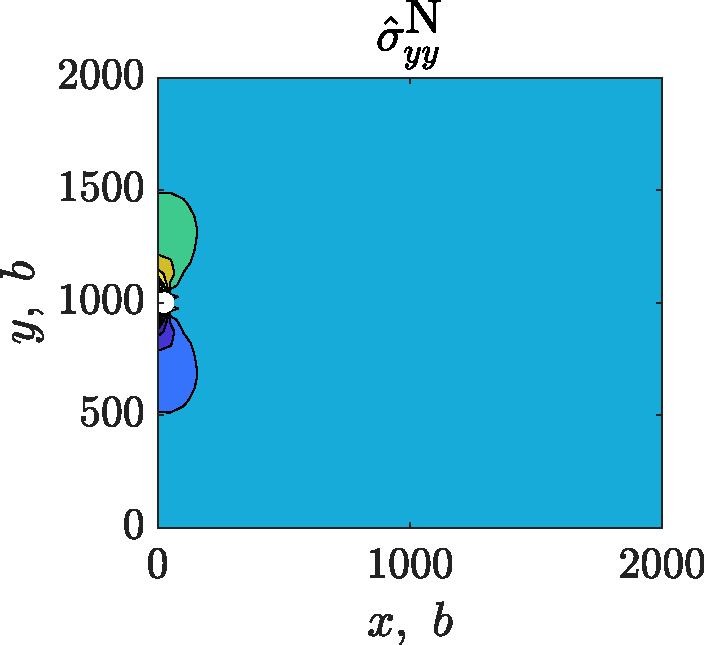
\includegraphics[width=0.25\linewidth]{syyNEperp_leg.pdf}}
    }~
    \subfloat{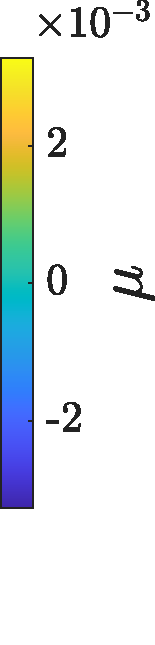
\includegraphics[height = 0.22\linewidth]{syyNAEperp_leg.pdf}}

    \hspace*{0.2cm}\subfloat[%$\hat{\sigma}_{xy}$.
        \hspace{-0.8cm}\label{sf:sxyeperp}]
    {
        {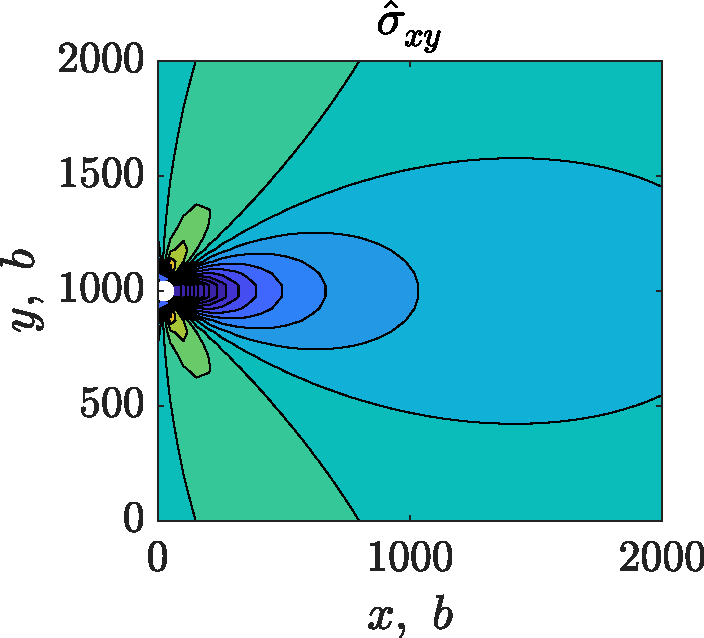
\includegraphics[width=0.25\linewidth]{sxyEperp_leg.pdf}}
    }~
    \subfloat[%$\hat{\sigma}^\textrm{A}_{xy}$.
        \hspace{-0.8cm}\label{sf:sxyAeperp}]
    {
        {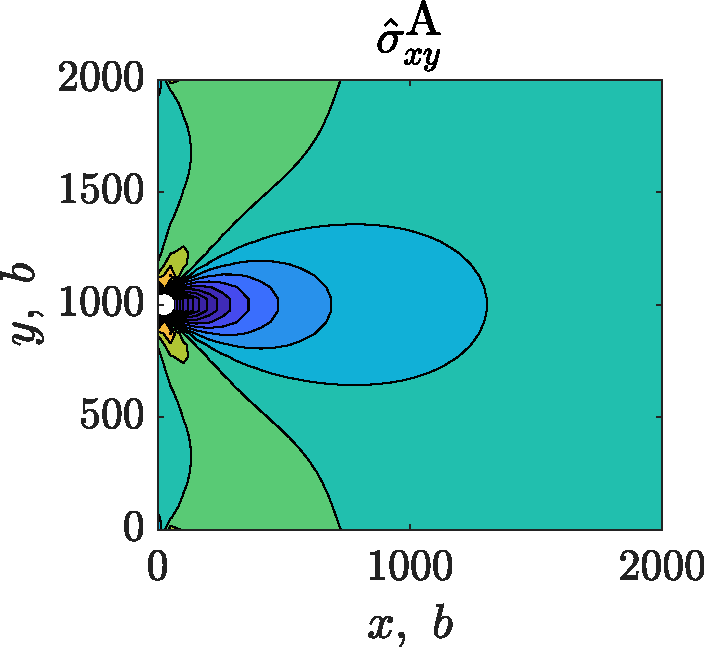
\includegraphics[width=0.25\linewidth]{sxyAEperp_leg.pdf}}
    }~
    \subfloat[%$\hat{\sigma}^\textrm{N}_{xy}$.
        \hspace{-0.8cm}\label{sf:sxyNeperp}]
    {
        {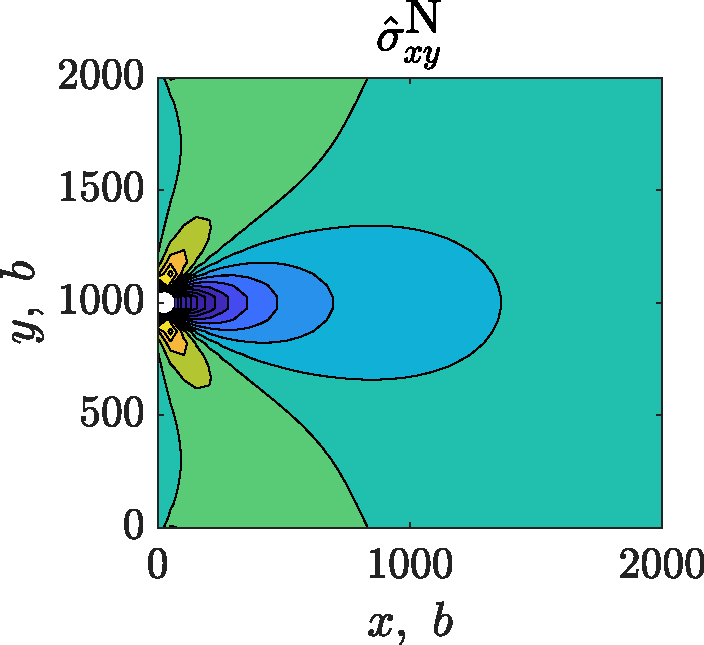
\includegraphics[width=0.25\linewidth]{sxyNEperp_leg.pdf}}
    }~
    \hspace*{-0.2cm}\subfloat{
        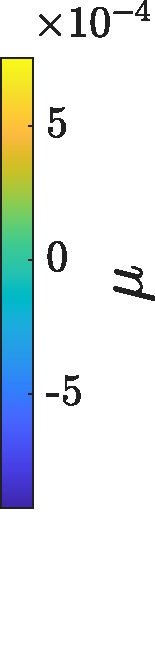
\includegraphics[height = 0.22\linewidth]{sxyNAEperp_leg.pdf}
    }

    \caption[Image stresses for an edge dislocation running parallel to a free surface with a Burgers vector perpendicular to the surface.]{Image stresses for an edge dislocation with $\vec{l} = [0 0 1]$, $\vec{b} = [1 0 0]$, where $a = 5$, with coordinates $(26,\, 1000)$, i.e. the centre of the first FE from the surface at $x=0$, and in the centre of the simulation box along the $y$-direction. (a), (e) and (i) are the stress fields for the infinite-domain solution, $\tns{\hat{\sigma}}$; (b), (f) and (j) are those obtaine from analytic tractions + FEM, $\tns{\hat{\sigma}}^{\textrm{A}}$; (c), (g) and (k) are those obtained using numeric tractions ($Q = 1$) + FEM, $\tns{\hat{\sigma}}^{\textrm{N}}$. (a) to (c) represent the $xx$; (e) to (g) the $yy$; and (i) to (k) the $xy$ components of the stress tensor.}
    \label{f:head_vs_ana_vs_num_eperp}
\end{figure}
As stated in \cref{ss:paperMethod}, tractions are used to calculate the image stresses resulting from the boundary conditions. We therefore compare the differences in image stresses resulting from numeric ($Q = 1$) and analytic traction calculations of both our implementations and how they compare to the infinite-domain, singular expressions in \cref{eq:imageStressAnalyticEdge1,eq:imageStressAnalyticEdge2,eq:imageStressAnalyticScrew}\footnote{Since the first term in each equation corresponds to the real stresses, we omit them to view the image stresses.}. The stress field comparisons for all three cases are found in \cref{f:head_vs_ana_vs_num_eperp,f:head_vs_ana_vs_num_epar,f:head_vs_ana_vs_num_screw}, where the dislocation is denoted by a white dot.

\begin{figure}[t]
    \centering
    \subfloat[%$\hat{\sigma}_{xx}$.
        \hspace{-0.8cm}\label{sf:sxxepar}]
    {
        {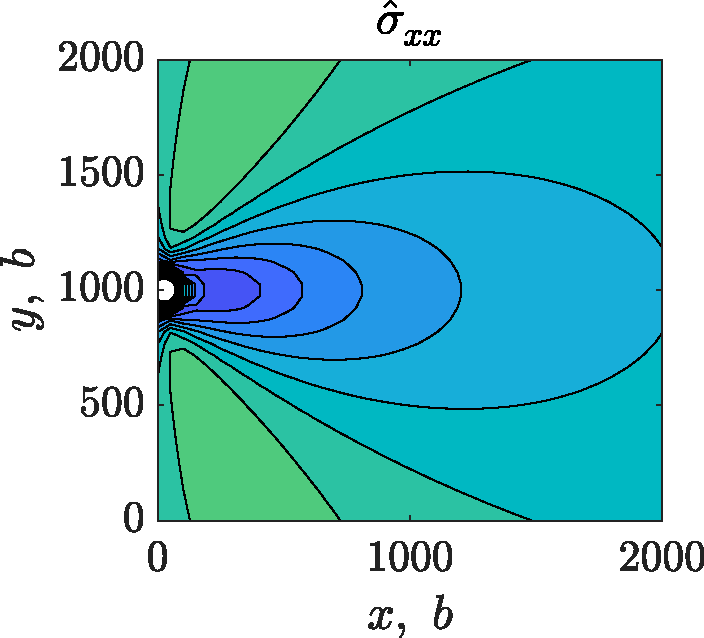
\includegraphics[width=0.25\linewidth]{sxxEpar_leg.pdf}}
    }~
    \subfloat[%$\hat{\sigma}^\textrm{A}_{xx}$.
        \hspace{-0.8cm}\label{sf:sxxAepar}]
    {
        {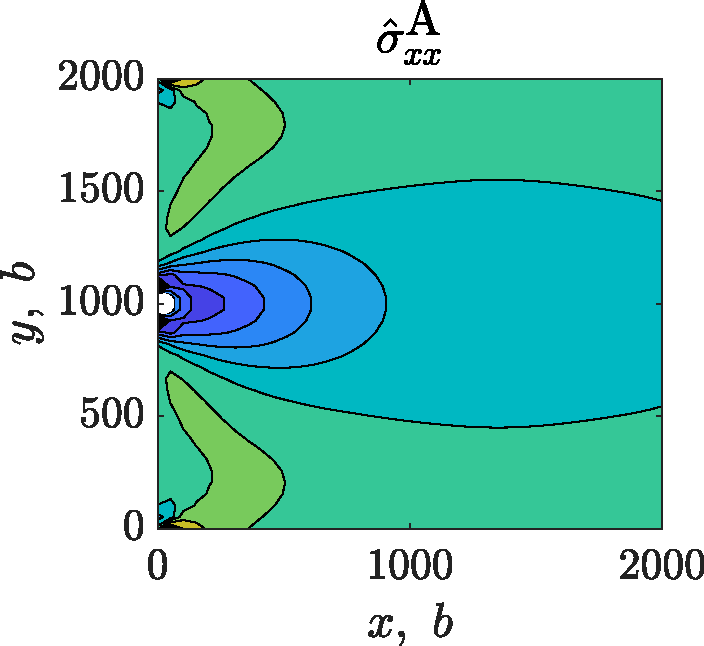
\includegraphics[width=0.25\linewidth]{sxxAEpar_leg.pdf}}
    }~
    \subfloat[%$\hat{\sigma}^\textrm{N}_{xx}$.
        \hspace{-0.8cm}\label{sf:sxxNepar}]
    {
        {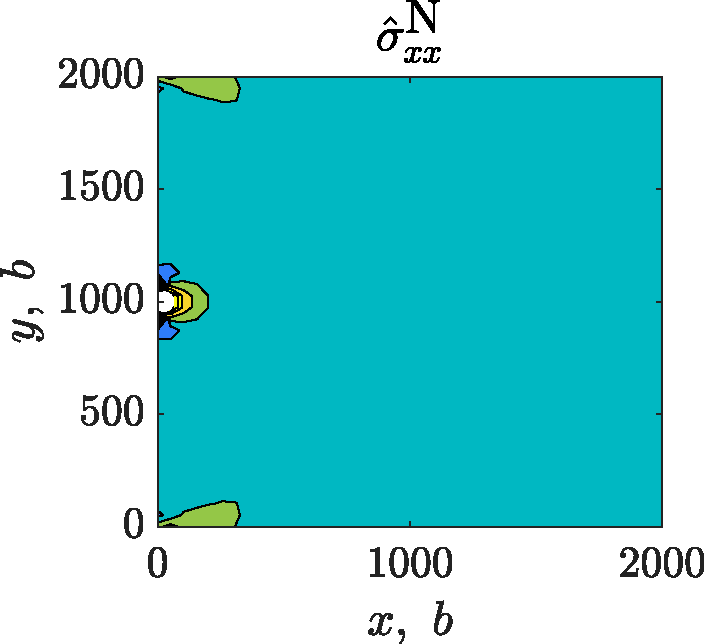
\includegraphics[width=0.25\linewidth]{sxxNEpar_leg.pdf}}
    }~
    \subfloat{
        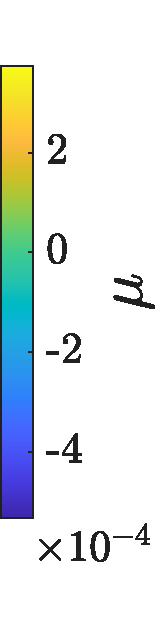
\includegraphics[height = 0.227\linewidth]{sxxNAEpar_leg.pdf}
    }

    \hspace*{0.3cm}\subfloat[%$\hat{\sigma}_{yy}$.
        \hspace{-0.8cm}\label{sf:syyepar}]
    {
        {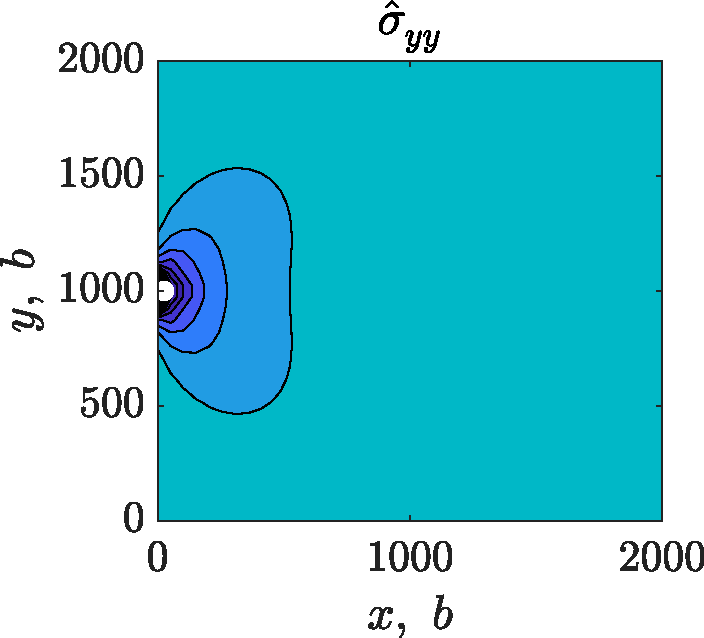
\includegraphics[width=0.25\linewidth]{syyEpar_leg.pdf}}
    }~
    \subfloat[%$\hat{\sigma}^\textrm{A}_{yy}$.
        \hspace{-0.8cm}\label{sf:syyAepar}]
    {
        {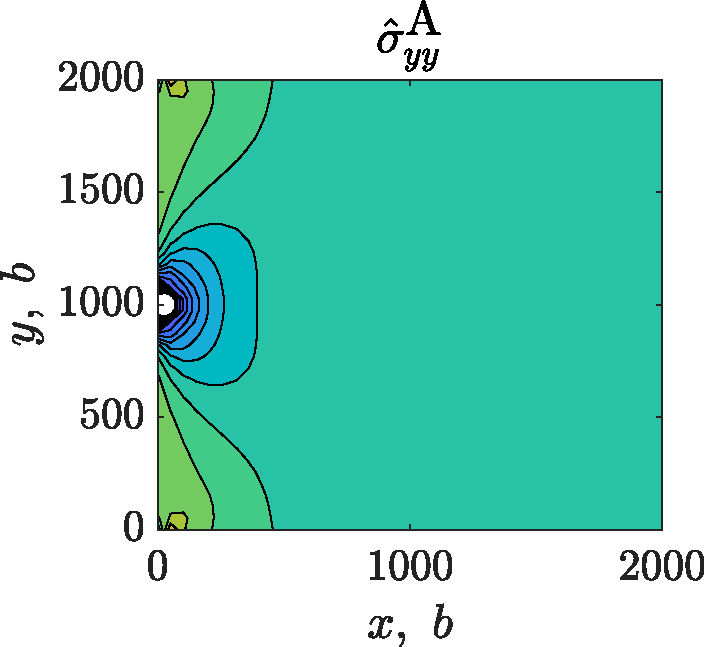
\includegraphics[width=0.25\linewidth]{syyAEpar_leg.pdf}}
    }~
    \subfloat[%$\hat{\sigma}^\textrm{N}_{yy}$.
        \hspace{-0.8cm}\label{sf:syyNepar}]
    {
        {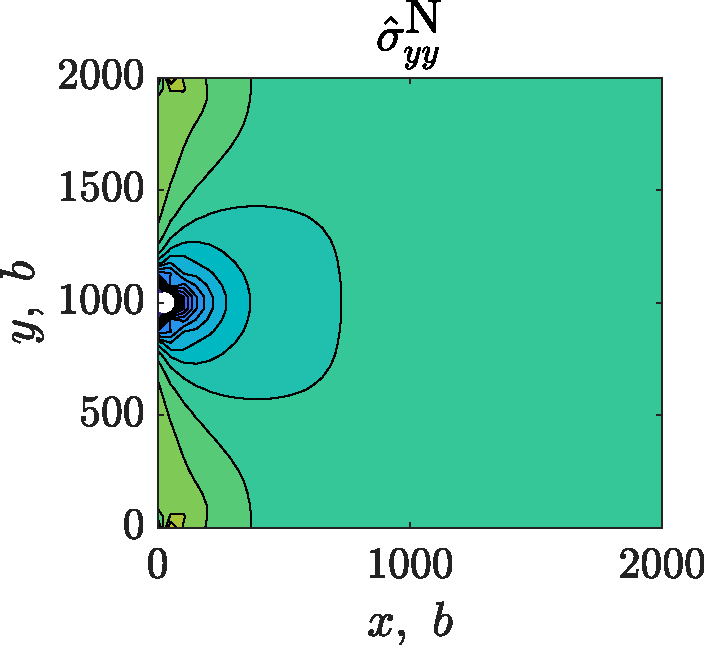
\includegraphics[width=0.25\linewidth]{syyNEpar_leg.pdf}}
    }~
    \subfloat{
        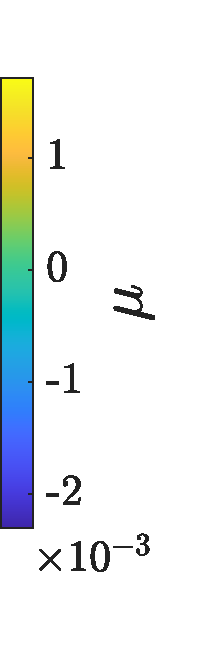
\includegraphics[height = 0.227\linewidth]{syyNAEpar_leg.pdf}
    }

    \hspace*{0.3cm}\subfloat[%$\hat{\sigma}_{xy}$.
        \hspace{-0.8cm}\label{sf:sxyepar}]
    {
        {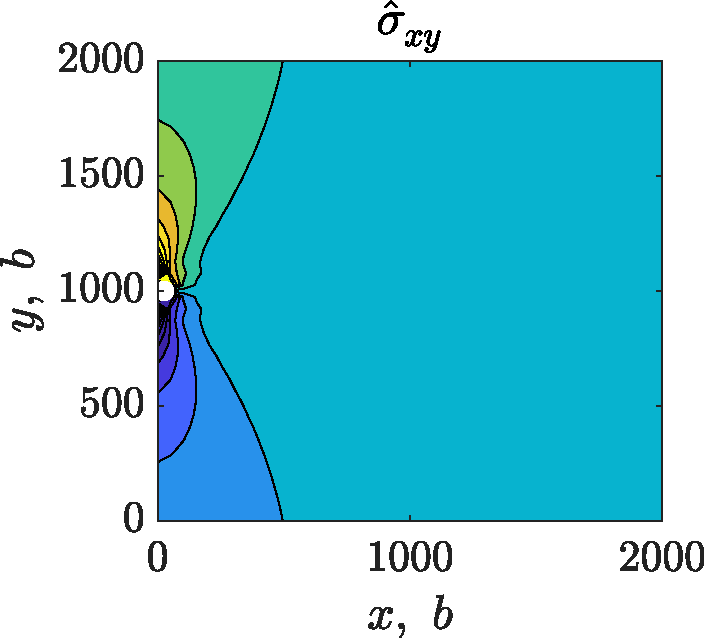
\includegraphics[width=0.25\linewidth]{sxyEpar_leg.pdf}}
    }~
    \subfloat[%$\hat{\sigma}^\textrm{A}_{xy}$.
        \hspace{-0.8cm}\label{sf:sxyAepar}]
    {
        {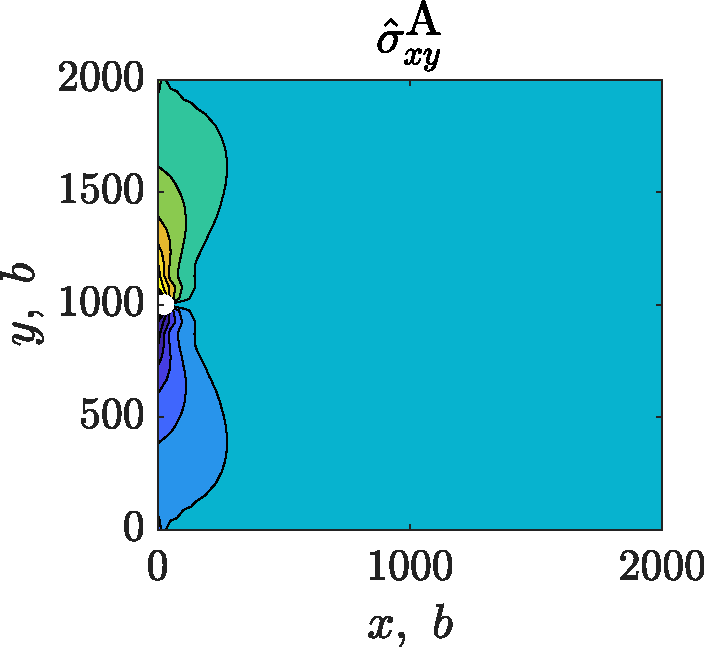
\includegraphics[width=0.25\linewidth]{sxyAEpar_leg.pdf}}
    }~
    \subfloat[%$\hat{\sigma}^\textrm{N}_{xy}$.
        \hspace{-0.8cm}\label{sf:sxyNepar}]
    {
        {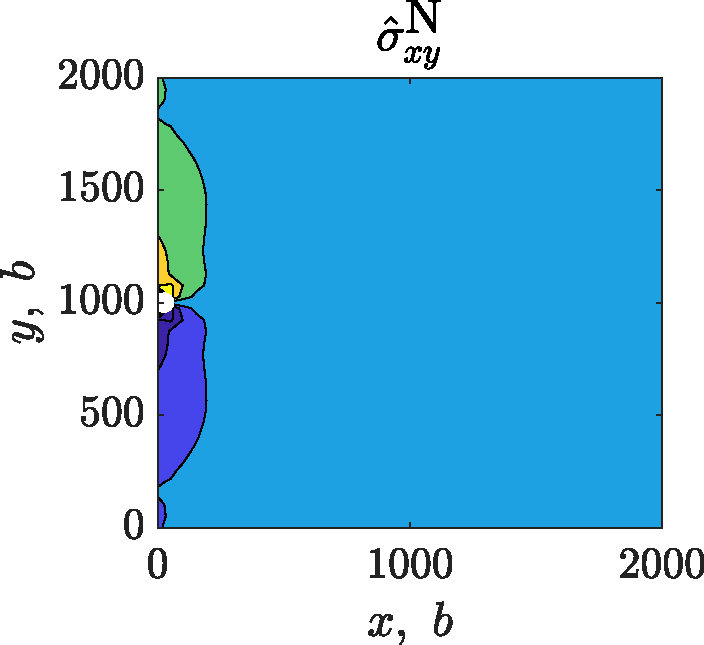
\includegraphics[width=0.25\linewidth]{sxyNEpar_leg.pdf}}
    }~
    \subfloat{
        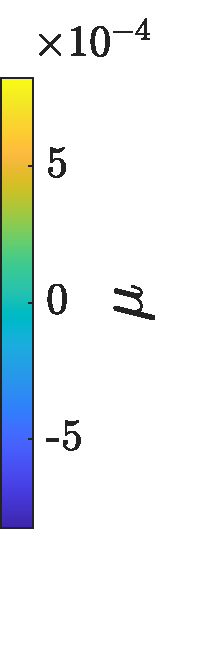
\includegraphics[height = 0.227\linewidth]{sxyNAEpar_leg.pdf}
    }

    \caption[Image stresses for an edge dislocation running parallel to a free surface with a Burgers vector parallel to the surface.]{Image stresses for an edge dislocation with $\vec{l} = [0\, 0\, 1]$, $\vec{b} = [0\, 1\, 0]$, where $a = 5$, with coordinates $(26,\, 1000)\, $, i.e. the centre of the first FE from the surface at $x=0$, and in the centre of the simulation box from top to bottom. (a), (e) and (i) are the stress fields for the infinite-domain solution, $\tns{\hat{\sigma}}$; (b), (f) and (j) are those obtaine from analytic tractions + FEM, $\tns{\hat{\sigma}}^{\textrm{A}}$; (c), (g) and (k) are those obtained using numeric tractions ($Q = 1$) + FEM, $\tns{\hat{\sigma}}^{\textrm{N}}$. (a) to (c) represent the $xx$; (e) to (g) the $yy$; and (i) to (k) the $xy$ components of the stress tensor.}
    \label{f:head_vs_ana_vs_num_epar}
\end{figure}
\Cref{f:head_vs_ana_vs_num_eperp} shows the stress fields corresponding to analytic expressions for image stress components, $\hat{\sigma}_{ij}$ in \cref{eq:imageStressAnalyticEdge1} where no superscript denotes the infinite-domain singular expressions, the $\textrm{A}$ superscript are the stresses calculated from analytic tractions and the $\textrm{N}$ superscript are those coming from numeric tractions where $Q = 1$ (same nomenclature in \cref{f:head_vs_ana_vs_num_epar,f:head_vs_ana_vs_num_screw}). The setup corresponds to the one described in \cref{f:headvstractionfem} where $\vec{b} = \vec{b}_{\textrm{e1}} = [1\, 0\, 0]$ and the dislocation is found at $(26, 1000)$.

It is clear edge effects play a role in the generated stresses. All three components have notable differences from the infinite-domain solutions resulting from the finite constraints, but the overall agreement between them all is quite good.

\begin{figure}
    \centering
    \subfloat[%$\hat{\sigma}_{xz}$.
        \hspace{-0.8cm}\label{sf:sxzscrew}]
    {
        {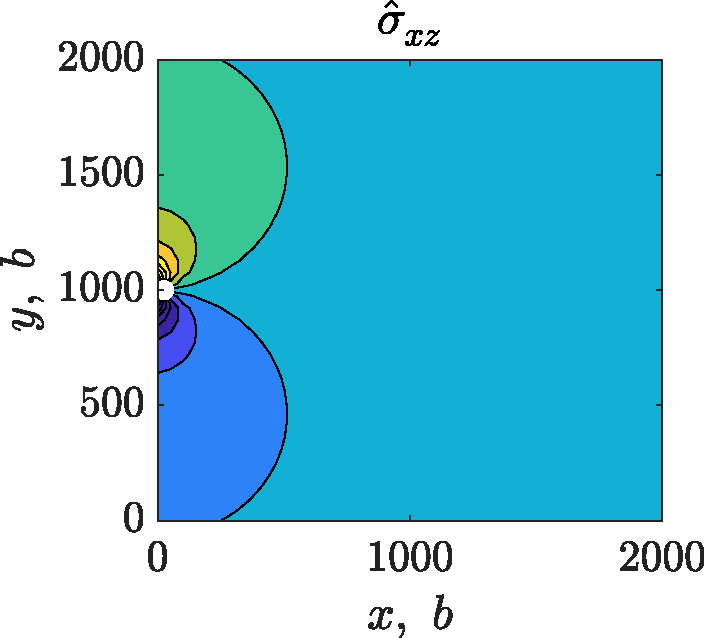
\includegraphics[width=0.25\linewidth]{sxzscrew_leg.pdf}}
    }~
    \subfloat[%$\hat{\sigma}^\textrm{A}_{xz}$.
        \hspace{-0.8cm}\label{sf:sxzAscrew}]
    {
        {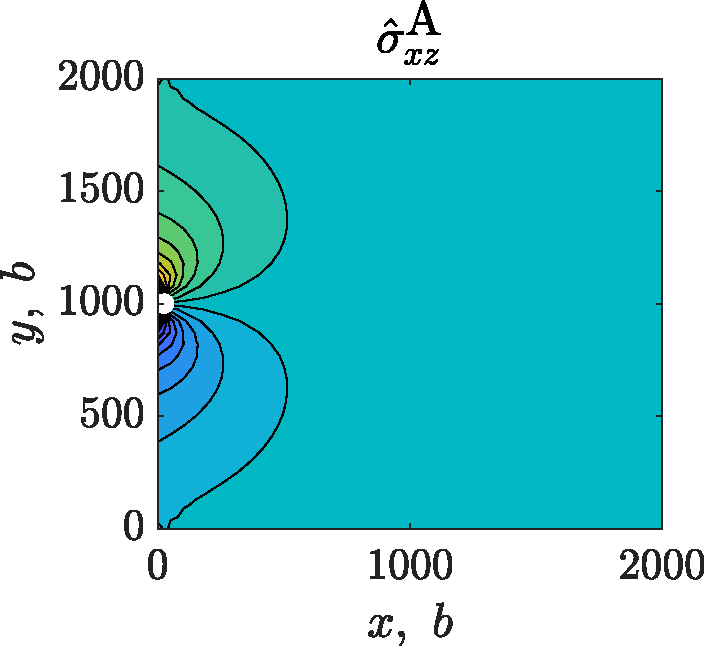
\includegraphics[width=0.25\linewidth]{sxzAscrew_leg.pdf}}
    }~
    \subfloat[%$\hat{\sigma}^\textrm{N}_{xz}$.
        \hspace{-0.8cm}\label{sf:sxzNscrew}]
    {
        {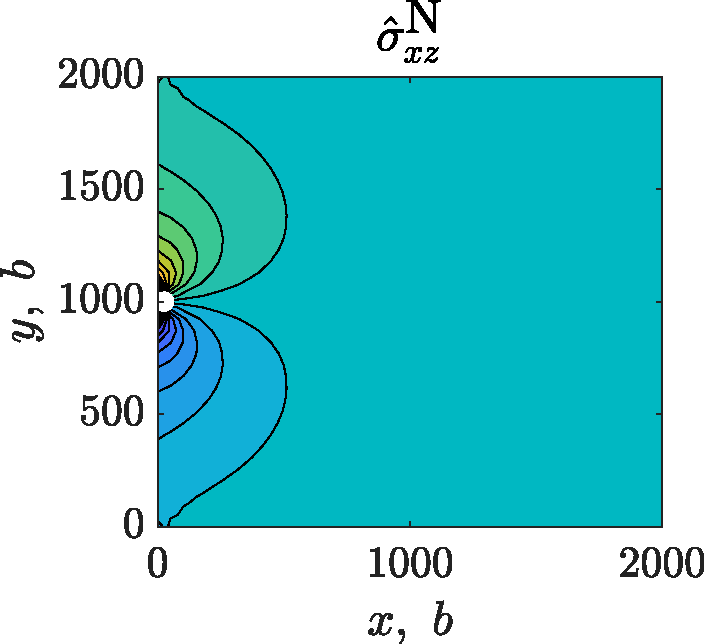
\includegraphics[width=0.25\linewidth]{sxzNscrew_leg.pdf}}
    }~
    \subfloat{
        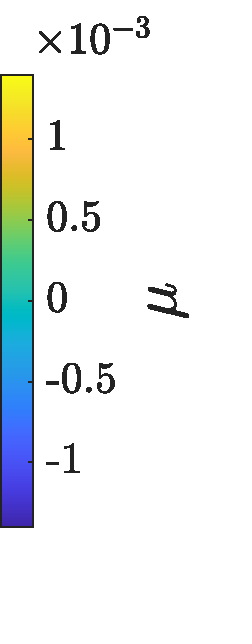
\includegraphics[height = 0.227\linewidth]{sxzNAscrew_leg.pdf}
    }

    \subfloat[%$\hat{\sigma}_{yz}$.
        \hspace{-0.8cm}\label{sf:szyscrew}]
    {
        {\includegraphics[width=0.25\linewidth]{syzscrew_leg.pdf}}
    }~
    \subfloat[%$\hat{\sigma}^\textrm{A}_{yz}$.
        \hspace{-0.8cm}\label{sf:syzAscrew}]
    {
        {\includegraphics[width=0.25\linewidth]{syzAscrew_leg.pdf}}
    }~
    \subfloat[%$\hat{\sigma}^\textrm{N}_{yz}$.
        \hspace{-0.8cm}\label{sf:syzNscrew}]
    {
        {\includegraphics[width=0.25\linewidth]{syzNscrew_leg}}
    }~
    \subfloat{
        \includegraphics[height = 0.227\linewidth]{syzNAscrew_leg.pdf}
    }
    \caption[Image stresses for a screw dislocation running parallel to a free surface.]{Image stresses for a screw dislocation with $\vec{l} = [0\, 0\, 1]$, $\vec{b} = [0\, 0\, 1]$, where $a = 5$, with coordinates $(26,\, 1000)\, $, i.e. the centre of the first FE from the surface at $x=0$, and in the centre of the simulation box from top to bottom.  (a) and (e) are the stress fields for the infinite-domain solution, $\tns{\hat{\sigma}}$; (b) and (f) are those obtaine from analytic tractions + FEM, $\tns{\hat{\sigma}}^{\textrm{A}}$; (c) and (g) are those obtained using numeric tractions ($Q = 1$) + FEM, $\tns{\hat{\sigma}}^{\textrm{N}}$. (a) to (c) represent the $xz$; (e) to (g) the $yz$.}
    \label{f:head_vs_ana_vs_num_screw}
\end{figure}
Things get markedly more interesting when looking at $\vec{b} = \vec{b}_{\textrm{e2}} = [0\, 1\, 0]$ in \cref{f:head_vs_ana_vs_num_epar} for a dislocation in the same place, $(26, 1000)$. Of particular note is $\hat{\sigma}_{xx}$, where a comparison between \cref{sf:sxxepar,sf:sxxAepar} and \cref{sf:sxxNepar} reveals one of the major issues with numeric tractions. If we look at the neighbourhood of the dislocation (just to the right), we will find a sign inversion i.e. yellow and green contours as opposed to purple and blue. As well as a drastically different isosurface shape. Image stresses like those can lead dislocations to behave quite differently than they should, particularly if the sign inversion also has a significantly different magnitude than the correct solution. Specifically, there is a region in the positive $x$-direction away from the dislocation where $\hat{\sigma}_{xx}$ is tensile rather than compressive. It is as absurd as a ship that floats by lowering the water level.

Perhaps the most evident deformation resulting from the displacement boundaries can be seen when $\vec{b} = \vec{b}_{\textrm{s}}$ in \cref{f:head_vs_ana_vs_num_screw}, where the lobes of the isolines are highly deformed when compared to the infinite-domain solutions. Though deformed, their familiar shape is still recognisable and both analytic and numeric tractions yield fairly similar fields.

\begin{figure}
    \centering
    \subfloat[$\hat{\sigma}_{xx}$.\label{sf:line_sxxperp}]
    {
        {\includegraphics[width=0.3\linewidth]{line_sxxEperp_leg.pdf}}
    }~
    \subfloat[$\hat{\sigma}_{yy}$.\label{sf:line_syyeperp}]
    {
        {\includegraphics[width=0.3\linewidth]{line_syyEperp_leg.pdf}}
    }~
    \subfloat[$\hat{\sigma}_{xy}$.\label{sf:line_sxyeperp}]
    {
        {\includegraphics[width=0.3\linewidth]{line_sxyEperp_leg.pdf}}
    }

    \subfloat[$\hat{\sigma}_{xx}$.\label{sf:line_sxxepar}]
    {
        {\includegraphics[width=0.3\linewidth]{line_sxxEpar_leg.pdf}}
    }~
    \subfloat[$\hat{\sigma}_{yy}$.\label{sf:line_syyepar}]
    {
        {\includegraphics[width=0.3\linewidth]{line_syyEpar_leg.pdf}}
    }~
    \subfloat[$\hat{\sigma}_{xy}$.\label{sf:line_sxyepar}]
    {
        {\includegraphics[width=0.3\linewidth]{line_sxyEpar_leg.pdf}}
    }

    \subfloat[$\hat{\sigma}_{xz}$.\label{sf:line_sxzscrew}]
    {
        {\includegraphics[width=0.3\linewidth]{line_sxzscrew_leg.pdf}}
    }~
    \subfloat[$\hat{\sigma}_{yz}$.\label{sf:line_syzscrew}]
    {
        {\includegraphics[width=0.3\linewidth]{line_syzscrew_leg.pdf}}
    }
    \caption[Line plots of the infinite domain, analytic and traction image stresses.]{Line plots of the image stresses of a dislocation at $(26, 1000)$ for a line going through $x = 103$ (start of the third element) for the analytic image stresses, as well as those calculated with numeric and analytic tractions. (a) to (c) correspond to $\vec{b} = \vec{b}_{\textrm{e1}}$, (d) to (f) $\vec{b} = \vec{b}_{\textrm{e2}}$ and (g) to (h) to $\vec{b} = \vec{b}_{\textrm{s}}$.}
    \label{f:line_head_vs_ana_vs_num}
\end{figure}
From \cref{f:head_vs_ana_vs_num_eperp,f:head_vs_ana_vs_num_epar,f:head_vs_ana_vs_num_screw} it seems like both analytic and numeric tractions are appropriate in most cases. At least at these scales, there is only one instance where numeric tractions yield very incorrect results. That said, these can have a significant impact on simulations, particularly those where multiple dislocations interact with surfaces in close proximity with one another.

\begin{figure}
    \centering
    \subfloat[\hspace{-0.8cm}\label{sf:sxxepar2}]
    {
        {\includegraphics[width=0.25\linewidth]{sxxEpar3_leg.pdf}}
    }~
    \subfloat[\hspace{-0.8cm}\label{sf:sxxAepar2}]
    {
        {\includegraphics[width=0.25\linewidth]{sxxAEpar3_leg.pdf}}
    }~
    \subfloat[\hspace{-0.8cm}\label{sf:sxxNepar2}]
    {
        {\includegraphics[width=0.25\linewidth]{sxxNEpar3_leg.pdf}}
    }
    ~
    \subfloat
    {
        {\includegraphics[height=0.227\linewidth]{sxxNAEpar3_leg.pdf}}
    }

    \subfloat[\hspace{-0.8cm}\label{sf:sxxepar11}]
    {
        {\includegraphics[width=0.25\linewidth]{sxxEpar11_leg.pdf}}
    }~
    \subfloat[\hspace{-0.8cm}\label{sf:sxxAepar11}]
    {
        {\includegraphics[width=0.25\linewidth]{sxxAEpar11_leg.pdf}}
    }~
    \subfloat[\hspace{-0.8cm}\label{sf:sxxNepar11}]
    {
        {\includegraphics[width=0.25\linewidth]{sxxNEpar11_leg.pdf}}
    }~
    {
    {\includegraphics[height=0.227\linewidth]{sxxNAEpar11_leg.pdf}}
    }

    \subfloat[\hspace{-0.8cm}\label{sf:sxxepartot2}]
    {
        {\includegraphics[width=0.25\linewidth]{sxxEparTot3_leg.pdf}}
    }~
    \subfloat[\hspace{-0.8cm}\label{sf:sxxAepartot2}]
    {
        {\includegraphics[width=0.25\linewidth]{sxxAEparTot3_leg.pdf}}
    }~
    \subfloat[\hspace{-0.8cm}\label{sf:sxxNepartot2}]
    {
        {\includegraphics[width=0.25\linewidth]{sxxNEparTot3_leg.pdf}}
    }~
    {
    {\includegraphics[height=0.227\linewidth]{sxxNAEparTot3_leg.pdf}}
    }

    \subfloat[\hspace{-0.8cm}\label{sf:sxxepartot11}]
    {
        {\includegraphics[width=0.25\linewidth]{sxxEparTot11_leg.pdf}}
    }~
    \subfloat[\hspace{-0.8cm}\label{sf:sxxAepartot11}]
    {
        {\includegraphics[width=0.25\linewidth]{sxxAEparTot11_leg.pdf}}
    }~
    \subfloat[\hspace{-0.8cm}\label{sf:sxxNepartot11}]
    {
        {\includegraphics[width=0.25\linewidth]{sxxNEparTot11_leg.pdf}}
    }
    ~
    {
    {\includegraphics[height=0.227\linewidth]{sxxNAEparTot11_leg.pdf}}
    }
    \caption[Convergence of the image and total stresses as a function of distance from the free surface.]{Stresses for an edge dislocation with $\vec{l} = [0\, 0\, 1]$, $\vec{b} = [0\, 1\, 0]$. Subfigures (a) to (g) show image stresses; (h) to (m) show total stresses. In subfigures (a) to (c) and (h) to (j) the dislocation is found at $(77,\, 1000)$; in (e) to (g) and (k) to (m) the dislocation is at $(487,\, 1000)$.}
    \label{f:head_vs_ana_vs_num_epar2to11}
\end{figure}
We also produced line plots to better show how the stress fields deviate from one another. \Cref{f:line_head_vs_ana_vs_num} shows line plots through the line $x = 103$ for a dislocation at $(26, 1000)$. \Cref{sf:line_sxxperp,sf:line_syyeperp,sf:line_sxyeperp} correspond to $\vec{b} = \vec{b}_{\textrm{e1}}$, \cref{sf:line_sxxepar,sf:line_syyepar,sf:line_sxyepar} to $\vec{b} = \vec{b}_{\textrm{e2}}$ and \cref{sf:line_sxzscrew,sf:line_syzscrew} to $\vec{b} = \vec{b}_{\textrm{s}}$. Here, the singular nature of the infinite-domain solutions is evidenced by the sharp spikes in its stresses. In general, the non-singular formulation smoothes out the stress line plots. However, there are a few instances where the numeric tractions lead to larger spikes than even the infinite-domain solutions such as in \cref{sf:line_sxxepar}. Again, the general shape of the line plots is the same but the tendancy for numerical tractions to spike under specific circumstances is evident in almost every case.

\begin{figure}
    \centering
    \subfloat[$\hat{\sigma}_{xx}$.\label{sf:line_sxxepar2}]
    {
        {\includegraphics[width=0.3\linewidth]{line_sxxEpar3.pdf}}
    }~
    \subfloat[$\hat{\sigma}_{xx}$.\label{sf:line_syyepar11}]
    {
        {\includegraphics[width=0.3\linewidth]{line_sxxEpar11_leg.pdf}}
    }

    \subfloat[$\sigma_{xx}$.\label{sf:line_sxxeparTot2}]
    {
        {\includegraphics[width=0.3\linewidth]{line_sxxEparTot3_leg.pdf}}
    }~
    \subfloat[$\sigma_{xx}$.\label{sf:line_sxxeparTot11}]
    {
        {\includegraphics[width=0.3\linewidth]{line_sxxEparTot11_leg.pdf}}
    }

    \caption[Line plots showing the convergence of the image and total stresses as a function of distance from the free surface.]{Line plots corresponding to \cref{f:head_vs_ana_vs_num_epar2to11}. (a) and (c) are of the image stresses; (b) and (d) are of total stresses. (a) and (b) are of a dislocation at $(77,\, 1000)$, taken along the line $x = 103$. (b) and (d) are of a dislocation at $(487,\, 1000)$, taken along the line $x = 513$.}
    \label{f:line_head_vs_ana_vs_num_epar2to11}
\end{figure}
To show the convergence in methods we also show stress fields in \cref{f:line_head_vs_ana_vs_num_epar2to11} and line plots \cref{f:line_head_vs_ana_vs_num_epar2to11} of the image and total stress fields as an edge dislocation with $\vec{b} = \vec{b}_{\textrm{e2}}$ moves from $(77,\, 1000)$ to  $(487,\, 1000)$. The line plots are taken from the second closest set of nodes in the positive $x$-direction i.e. at $x = 103,\, 513$.

Notice that the image stresses in \cref{sf:sxxepar2,sf:sxxAepar2,sf:sxxNepar2} are all very close to \cref{sf:sxxNepar}, which is the stress field calculated via numerical tractions for a dislocation that is slightly closer to the surface. Essentially, the numerical tractions over or underestimated a set of forces something that become the dominant contributors as the dislocation moves away from the surface.

From \cref{f:head_vs_ana_vs_num_epar2to11,f:line_head_vs_ana_vs_num_epar2to11} it can be observed that both analytic and numeric tractions converge to similar shapes to each other as expected. However it also becomes clear that the infinite-domain solution is not totally accurate for image stresses in finite domains due to edge effects.

Lastly, to show how much numeric tractions can affect a result, \cref{f:simulation} shows a few snapshots of the simulation described in \cref{ss:paperMethod}. The figures shown are not at equivalent times because the simulations using numeric tractions ran indefenitely. The line tension equilibrated with the image forces on the traction-free surface, preventing the dislocation from exiting and keeping it oscillating in a local energy minimum. The simulation using analytic tractions ended when the dislocation completely exited the surface as expected. It is feasable that at some point, the simulation using numeric tractions could jump out of the local minimum due to some spike in the tractions, but the last image was taken for a simulation time approximately 20 times greater than it took the one using analytic tractions to end when the dislocation fully exited the box.
\begin{figure}
    \subfloat[Analytic tractions $t = 0$.]
    {
        {\includegraphics[width=0.3\linewidth]{analytic_0.pdf}}
    }~
    \subfloat[Analytic tractions mid simulation.]
    {
        {\includegraphics[width=0.3\linewidth]{analytic_50.pdf}}
    }~
    \subfloat[Analytic tractions end.]
    {
        {\includegraphics[width=0.3\linewidth]{analytic_66.pdf}}
    }

    \subfloat[Numeric tractions $t = 0$.]
    {
        {\includegraphics[width=0.3\linewidth]{numeric_0.pdf}}
    }~
    \subfloat[Numeric tractions mid simulation.]
    {
        {\includegraphics[width=0.3\linewidth]{numeric_78.pdf}}
    }~
    \subfloat[Numeric tractions $t \to \infty$.]
    {
        {\includegraphics[width=0.3\linewidth]{numeric_156.pdf}}
    }
    \caption[Unloaded simulations using analytic and numeric tractions.]{Progression of simulations using both traction calculation methods.}
    \label{f:simulation}
\end{figure}

\subsection{Conclusion}\label{ss:paperConclusion}

Often the effects of tractions on a simulation can be quite subtle if things do not go catastrophically wrong, but a quick and easy way of seeing how the numeric tractions have a tendancy to spike and invert sign (as in \cref{sf:line_sxxepar}) is to pause a simulation while its running and scatter plot the numeric tractions v.s. analytic ones. The plot will show a positive correlation---as the sign inversions in numeric tractions are relatively rare events---but whichever axis corresponds to the numeric tractions will have the largest range. Using proportional axes makes the differences quite evident even at a quick glance as the aspect ratio will be far from 1:1.

In other parts of our work, we have noted that despite the analytic tractions taking approximately 10 times longer to compute than numerically calculated tractions with $Q = 1$ (which agrees with the findings in \cite{analytic_tractions}), yield more stable and ultimately faster simulations. Even simple simulations are typically faster when using analytic tractions over numeric ones. This was not the case with the simulation we show here, but the numeric tractions led to a hung simulation, which we have found is quite common. The margin by which using analytic tractions leads to faster overall simulations grows as simulation complexity increases. Only the simplest simulations initially benefit from numeric tractions but this often decreases and reverses as the simulation advances. Another fortunate side effect of more accurate tractions is the fact that fewer dislocation segments are generated during simulations, which \citet{bromage2018calculating} found when correctly accounting for the displacements generated by dislocations.

Given our findings, we cannot recommend using numeric tractions when analytic ones are available. The losses in computational speed that result from moving from one to the other are more than made up for by the fewer topological operations, fewer generated segments, and more accurate velocities. All of which result in fewer calculations of segment-segment interactions, fewer collisions, larger timesteps and ultimately cleaner simulations that run into fewer snags along the way.

There is a case however, for combining both approaches in larger scale simulations. Since both numeric and analytic tractions converge to the same value as the dislocation-surface distance increases, a hybrid approach may possibly be undertaken without many negatives. Furthermore, \cite{analytic_tractions} also derived a Taylor series expansion of the solutions which can be used in cases where the dislocation-surface distance is large. These may be worth exploring in larger scale simulatios. However, in the types of systems we model, other parts of our model tend to be much more rate-limiting than tractions. As such, we have all but ceased to use numeric tractions in our work.

\section{GPU parallelisation of analytic tractions}\label{s:parallel}
% add this figure https://www.researchgate.net/figure/Typical-NVIDIA-GPU-architecture-The-GPU-is-comprised-of-a-set-of-Streaming_fig1_236666656

Graphics Processing Units (GPUs) have been leveraged by digital art, animation studios and gaming companies since the 1990s to offload repetitive, grid-based mathematical computations away from the Central Processing Units (CPUs). These operations are usually very computationally cheap, require minimal logic, and do not need more than single precision (32-bit) arithmetic \cite{gpu1,gpu2,gpu3}, in fact, increases in accuracy would get lost in the RGB channel regardless. As such, GPUs evolved primarily to efficiently perform lightweight operations on vast amounts of 32-bit data. As such, their memory buses are extremely fast and and their processors very minimalistic.

It wasn't until much later that engineers and scientists picked up on the potential of GPUs \cite{gpu_comp,mixedPrecFEM,jia2014gpu}. Fields where lower precision is advantageous---because it increases the signal to noise ratio, or real-world tolerances exceed the in-silico precision---such as data science, civil engineering and image/signal processing, first leveraged this technology. In fact, many big data applications operate on half and some even go as low as quarter precision simply due to the low sensitivity, large amount of noise and vast quantities of data \cite{pagerank}.

NVidia has spearheaded the development and adoption of scientific-computing and high performance computing (HPC) GPUs with the development of their propriatory Compute Unified Device Architecture, CUDA technology. They now produce a wide range of GPUs tailored for scientific applications. These have specialised architecture \cite{nvidia}.
\begin{itemize}
    \item Tensor modules for fast, piecewise matrix multiplication.
    \item Larger but slower memory buses mean higher concurrent resource use because scientific computations are expensive, so it is better to have them work through a lot of data while more memory is being fetched, rather than fecthing small amounts of memory really quickly but having to wait for the processors to finish their computation.
    \item Expanded precision capabilities.
    \item Specialised registers, specialised heirarchical memory architecture, etc.
\end{itemize}

For all their advantages, parallel algorithms are fundamentally different to serial ones. In particular the way GPUs differ from CPUs makes it a non-trivial task to properly parallelise an algorithm. Doing so poorly can result in decreased performance, particularly when using high performace/scientific computing cards. There is also the issue of scaling, whereby the cost of utilising the GPU may not be worth paying until a certain computation size. In this section, we detail the work, results and conclusions of parallelising the analytic traction calculation.

\subsection{Data Mapping}

A cache is a store of memory used to reduce the cost of accessing data from the main memory. CPUs and GPUs have cache heirarchies designed to progressively get smaller and faster the closer they are to the processor. This reduces the average cost of accessing data because the missing data can be looked for in progressively higher cache levels. It is important to know that caches operate as single units, meaning that every time a processor needs data that is not found in a cache (cache miss), the whole cache needs to be updated. This means that every time there is a cache miss, any operations dependent on the missing data have to wait until the new data arrives. As processors have gotten faster, memory speeds have not kept up. As a result, minimising the ratio of cache misses to cache hits has become an important aspect of optimising software applications \cite{cpuMemDiv,gpuMemDiv}. Optimising cache use is of particular importance in GPUs.

The increasingly divergent speeds of processors and memory, are the reason why scientific computing GPUs opt for larger but slower memory buses. In properly written software, this feature decreses the time spent waiting for a processor to finish whilst the data is ready \cite{gpuCache,sharedCache,gpuMemDiv2}. Tnstead the infrastructure and cost associated with faster memory can be better utilised on more processing power. However, in improperly written code, the cache miss to hit ratio will be large. Non-scientific applications can get away with this to an extent, because memory buses are fast and computational cost is low. But for scientific applications---and in particular when using specialised GPUs---this can be catastrophic for performance.

In NVidia GPUs, ``coalesced memory access'' is when, a single cache line contains all the data needed by a ``warp''---a collection of 32 threads which operate ``simultaneously'' as a single unit on separate pieces of data---to carry out an instruction/process. This is not always possible because it is problem-dependent, so usually the best we can do is ensure there are no unecessary memory fetches by arranging simultaneously-used data in a contiguous manner. \Cref{f:mem_access} is a simple example of this.
\begin{figure}
    \centering
    \includegraphics[width=0.8\linewidth]{mem_access.pdf}
    \caption[Memory access patterns.]{Memory access patterns. Arrows are threads in a warp simultaneously requesting access to memory from the cache. All processors work simultaneously, so they can only proceed until every one of them has the necessary data.}
    \label{f:mem_access}
\end{figure}

Since threads in a warp behave as a single unit, they hang until every other thread in the warp has the data it needs to execute the next instruction. Under a strided memory access pattern, this happens more often than if the data were contiguously accessed. Furthermore, cache usage optimisation heuristics have the task of deciding what memory to bring in order to minimise future cache misses. Under a contiguous memory access model, this done by simply placing the first missing item as the first item in the next cache line. However, even in the simple example of strided memory access shown in \cref{f:mem_access}, it's easy to see how this is suboptimal. To start with, a new cache line is needed for the for the second iteration instead of the third, as it would be if the access pattern were contiguous. Then, the new cache line could start with $h_y$ and still work for the second iteration, but then a new cache line would be needed for the third. However, grabbing the first missing item as the first item of the cache line used in the second iteration means going back down for the third iteration. In fact, the optimum strategy in this case would be to start the cache line for the second iteration on the third item, $h_z$, in the cache line for the first iteration.

As a result, we have to be extremely careful when mapping CPU (host) memory, arranged to be advantageous for serial access (and therefore human intuition), to device (GPU) memory, arranged for parallel access.

\subsection{Parallelisation schemes}

The traction calculation is $\mathcal{O}(MN)$, where $M$ is the number of surface elements and $N$
the number of segments. As such, there are two first order parallelisation strategies. Parallelising over elements and looping over segments; parallelising over segments and looping over elements. And two second order parallelisation strategies. Parallelising over elements and subparallelising over segments and vice-versa. However, higher order parallelisations are usually disadvantageous unless the problem is very computationally cheap because there is more competition for parallel resource use. We only implemented both first order parallelisations. There cannot be a parallelisation over nodes as the unit problem is a single surface element and dislocation segment.

Both first order parallelisations have similar performances, but parallelising over dislocations have better scaling as simulations advance because the number of surface elements is constant while the number of dislocation segments tends to increase. The choice of parallelisation will depend on the relative amounts of surface elements to dislocation segments.

The algorithm for mapping from the objects to be parallelised over from host (CPU) to device (GPU) memory is the same in either case. The only thing that changes is that surface elements have 4 nodes and dislocation segments have 2. If parallelising over dislocation segments, the Burgers vector also needs to be mapped in the same manner, but it is equivalent to having a single `node'. The mapping is as follows,
\begin{subequations}\label{eq:hostDeviceElementMap}
    \begin{align}
        \vec{X}_{en}        & \coloneqq	\left[x_{en},\, y_{en},\, z_{en}\right]                                                     \\
        \vec{X}_{(1\to E)n} & \mapsto 	\vec{X}_{n} \nn
        \vec{X}_{n}         & \coloneqq	\left[x_{1n},\, y_{1n},\, z_{1n},\ldots,x_{En},\, y_{En},\, z_{En}\right]\label{seq:xn_arr} \\
        \vec{X}_{1\to N}    & \mapsto	\vec{X}\nn
        \vec{X}             & \coloneqq
        \begin{aligned}
             & \left[x_{11},\, \ldots,\, x_{E1},\, x_{12},\, \ldots,\, x_{E2},\, \ldots,\, x_{1N},\, \ldots,\, x_{EN}, \right.      \\
             & \left.\,y_{11},\, \ldots,\, y_{E1},\, y_{12},\, \ldots,\, y_{E2},\, \ldots,\, y_{1N},\, \ldots,\, y_{EN}, \right.    \\
             & \left.\,z_{11},\, \ldots,\, z_{E1},\, z_{12},\, \ldots,\, z_{E2},\, \ldots,\, z_{1N},\, \ldots,\, z_{EN}  \right]\,.
        \end{aligned}
    \end{align}
\end{subequations}
where $ e $ is the element to be mapped, $ n $ the node number, $ E $ the total number of elements and $N$ the total number of nodes per element.

\begin{figure}
    \centering
    \includegraphics[width=\linewidth]{parallel_labels.pdf}
    \caption[Linear rectangular surface element mapping.]{Each linear rectangular surface element is mapped to one thread.}
    \label{f:paraLabel}
\end{figure}
For a set up like \cref{f:paraLabel}, parallelising over the surface elements with node labels corresponding to \cref{f:force_lin_rect}, $\vec{x_1}$, $\vec{x_2}$, $\vec{x_3}$ and $\vec{x_4}$ yields,
\begin{align}\label{eq:fcne_eg}
    \vec{X} & = \begin{aligned}
        \left[\underbrace{h_{x},\, i_{x},\, f_{x},\, g_{x}}_{\vec{x_{1}}},\,
        \underbrace{a_{x},\, b_{x},\, i_{x},\, h_{x}}_{\vec{x_{2}}},\,
        \right.  & \underbrace{i_{x},\, d_{x},\, e_{x},\, f_{x}}_{\vec{x_{3}}},\,
        \underbrace{b_{x},\, c_{x},\, d_{x},\, i_{x}}_{\vec{x_{4}}},              \\
        \ldots~y & \textrm{-coord}~\ldots,                                        \\
        \ldots~z & \textrm{-coord}~\ldots]\,.
    \end{aligned}
\end{align}

Whether the parallelisation is done over dislocation line segments or surface elements, the item that wasn't parallelised over must also be mapped such that it can be contiguously accessed by the GPU. However this just means merging arrays in a very simple manner,
\begin{subequations}\label{eq:fnce}
    \begin{align}
        \vec{X}_{en}        & \coloneqq \left[x_{en},\, y_{en},\, z_{en}\right]                                                    \\
        \vec{X}_{(1\to E)n} & \mapsto \vec{X}_{n} \nn
        \vec{X}_{n}         & \coloneqq \left[x_{1n},\ldots,\, x_{En},\, y_{1n},\ldots,\, y_{En},\, z_{1n},\ldots,\, z_{En}\right] \\
        \vec{X}_{1\to N}    & \mapsto \vec{X}\nn
        \vec{X}             & \coloneqq
        \begin{aligned}
            \left[x_{11},\ldots,\, x_{E1},\, y_{11},\right. & \ldots,\, y_{E1},\, z_{11},\ldots,\, z_{E1}              \\
            ,                                               & \ldots,                                                  \\
            x_{1M},\ldots,\, x_{EN},\, y_{1N},              & \left.\ldots,\, y_{EN},\, z_{1N},\ldots,\, z_{EN}\right]
        \end{aligned}
    \end{align}
\end{subequations}
In a similar vein to \cref{eq:fcne_eg}, using \cref{eq:fnce} to map the data yields,
\begin{align}\label{eq:fnce_eg}
    \vec{X} & = \begin{aligned}
         & \left[\underbrace{h_{x},\, i_{x},\, f_{x},\, g_{x},\,
            h_{y},\, i_{y},\, f_{y},\, g_{y},\,
        h_{z},\, i_{z},\, f_{z},\, g_{z}}_{\mathbf{x_{0}}}\right.,  \\
         & ~\ldots~\mathbf{x_{1}},\, xyz\textrm{-coords}~\ldots,    \\
         & ~\ldots~\mathbf{x_{2}},\, xyz\textrm{-coords}~\ldots,    \\
         & ~\ldots~\mathbf{x_{3}},\, xyz\textrm{-coords}~\ldots]\,.
    \end{aligned}
\end{align}

\subsection{Maximising performance}

In order to maximise performance after properly mapping memory to the GPU we have to minimise hang time. A good rule of thumb is to try optimising cache use. Full cache line utilisation (coalesced memory access) is achieved if cache lines can accomodate $ l $ entries given by \cref{eq:opt_cache_len_bcne},
\begin{align}
    \label{eq:opt_cache_len_bcne}
    l =
    \begin{cases}
        a \times N \times E\,,                & \quad a > 0 \in \mathbb{N}                                                \\
        \textrm{or}                                                                                                       \\
        \dfrac{1}{2^{a}} \times N \times E\,, & \quad a \geq 0 \in \mathbb{N},\, N \times E \equiv 0\; (\bmod\; 2^{a})\,,
    \end{cases}
\end{align}
where $a$ is the number of entries, $N$ the number of nodes and $E$ the number of elements. This can be achieved by making use of the flexibility afforded by the NVidida architecture. Every GPU has various collections of warps called Streaming Microprocessors (SMs). Each SM is independent of other SMs, however, warps within an SM all share certain resources such as various levels of caches and schedulers. Each SM can be split into blocks of threads, all of which share some resources. The optimal usage entails finding the best block size (preferably a multiple of 32 to maximise thread usage, as the smallest unit of processing is a warp) for a particular problem. Each block as a dimension (the number of threads inside it), an index (there can be multiple blocks in a single SM), and each thread has an index that identifies it within its block. These values are used to index the global device memory. \Cref{f:parallel_exec} has an example of how this works for a block of two threads and a set up as described by \cref{f:paraLabel} and mapping by \cref{eq:hostDeviceElementMap}.
\begin{figure}
    \centering
    \includegraphics[width=\linewidth]{node_bmap.pdf}
    \caption[Sample parallel execution.]{Minimum working complete example of a thread block obtaining data from global memory, from parallelising over the four surface elements in \cref{f:paraLabel} and mapped by \cref{eq:hostDeviceElementMap}. $\vec{X_{a}^{b}}$ denotes a 1D array of length three containing the $ xyz $-coordinates of node $ a $ of element $ b $. Each thread concerns itself with only one element at a time. The dash-dot and dashed boxes represent cache lines for a thread block, the dotted line represents a memory fetch, and the dashed lines in $ \vec{X^{E}} $ represent steps of $ E $ entries (the start of the data for the next node of the element type we're dealing with). The memory operations are not shown twice to minimuse redundancy.}
    \label{f:parallel_exec}
\end{figure}

Realistically, this is extremely difficult to achieve, particularly in dynamic, non-conservative simulations such as discrete dislocation dynamics. So we also came up with two heuristics that aim to utilise as many computational resources as possible.
\begin{align}\label{eq:numThreads}
    T & = 32 \left\lceil\mod(n,\, T_{\rvar{max}} )/32 \right\rceil \\
    G & = \left\lceil (n + T - 1) / T \right\rceil\,,
\end{align}
where $n$ is the number of items to be parallelised (either surface elements or dislocation line segments), $T$ is the number of threads per block, $T_{\rvar{max}}$ is the maximum number of threads allowed in a block (GPU dependent) and $G$ is the total number of blocks. $G$ ensures the load gets distributed evenly across as many blocks as possible, and $T$ ensures each thread block is busy for the longest time possible between memory fetches.

\subsection{Solving parallelisation problems}

One of the things that can be missed during parallelisation is the fact that writing to global memory is asyncronous. This means that threads can race each other to write to global memory. Fortunately we avoided some of the more egregious issues because each unit problem is independent of the rest. However, the forces calculated independently accross threads have to be sequentially added to the overall force on each node. This is done with atomic operations, that force the threads to sequentially write their contributions to the global memory.

The second issue is that of the singularity when a dislocation segment is parallel to a surface, see \cref{eq:problem}.

The reason this is such an issue is because GPUs cannot branch. That is to say, every case of an if or case statement is executed regardless of whether a condition is met or not. The only difference is that the values are only stored if a condition is met. This means that cases as rare yet costly as these, disproportionatley impact performance. Parallelising over special cases is not worth the time because they are not common enough, so the best solution use the fact that GPUs and CPUs work asyncronously and have the GPU only store the data for non-special cases, while the CPU only calculated the contributions from the special cases. Both contributions are added back at the end.

\subsection{Results and conclusion}

\begin{figure}
    \centering
    \includegraphics[width=\linewidth]{speed_up.pdf}
    \caption[Parallel speedup on an NVidia GTX 750.]{Parallel speedup on an NVidia GTX 750.}
    \label{fig:parallel}
\end{figure}

One of the greatest disapointments of this project can be seen in \cref{fig:parallel}. It was produced using a linux workstation with an NVidia GTX 750 and an Intel Core i5-8500 @ 3.0 GHz. Both GPU and CPU are equally outdated so the comparison remains relatively fair insofar as other non-HPC set ups are concerned. That said, using a high performance GPU would help a great deal as CPUs have somewhat stagnated in comparison. Regardless it wouldn't help the root cause. The $x$-axis is scaled to $10^5$ dislocation segments. We have nowhere near the capacity to run a simulation with $10^5$ segments. The $\mathcal(O)(N^2)$ collision and segment-segment force algorithms and $\mathcal(O)(N!)$ separation prevent us from going much past $10^4$ segments. Moreover, \cref{fig:parallel} was obtained using only non-parallel segments, the code checking for parallel ones in the CPU was not even compiled. Therefore, the speed up is purely from the GPU. Unfortunately, checking for the special case means the CPU can lag behind the GPU in some scenarios, reducing the true gains by a noticeable margin.

While using the GPU-accelerated code does not actively hinder most simulations, it doesn't help much either. Larger simulations on more advanced hadware are sped up, but other processes slow them down before the computational gains can be realised.

The analytic traction calculation is particularly troublesome for parallelisation. Not only is it much more computationally intensive than what GPUs are normally used for, but also has disproportionately expensive and rare corner cases, and has an awkward unit problem that necesitates a lot of data. It is too far removed from the relatively simpler layouts of ``trivially'' parallelisable grid-based problems found in fluid dynamics, civil engineering and image processing that get so much out of GPU parallelisation.

The silver lining to this is that the parallelised code is close to optimal. So when the rest of the software and hardware catch up to the complexity presented by the analytic tractions, it'll be there to shine like it deserves.
\savearabiccounter
% 7533